% !TeX spellcheck = ru_RU
\documentclass[a4paper,12pt,russian]{extarticle}
\usepackage{extsizes}
\usepackage{cmap} % для кодировки шрифтов в pdf
\usepackage[section]{placeins}
\usepackage[T2A]{fontenc}
\usepackage[utf8]{inputenc}
\usepackage[russian]{babel}
\usepackage{slashbox}
\usepackage{graphicx} % для вставки картинок
\graphicspath{ {./figures/} }
\usepackage{amssymb,amsfonts,amsmath,amsthm} % математические дополнения от АМС
\usepackage{indentfirst} % отделять первую строку раздела абзацным отступом тоже
\usepackage[usenames,dvipsnames]{color} % названия цветов
\usepackage{makecell}
\usepackage{csquotes}
\usepackage{multirow} % улучшенное форматирование таблиц
\usepackage{ulem} % подчеркивания
\usepackage{titletoc}
\usepackage{tikz}
\usepackage{float}
\usetikzlibrary{chains,shapes.multipart}
\usetikzlibrary{shapes,calc}
\usetikzlibrary{automata,positioning}
\usepackage[left=3cm,right=1.5cm,
top=2cm,bottom=2cm,bindingoffset=0cm]{geometry}
\newtheorem{theorem}{Теорема}


\usepackage{listings}
\usepackage{xcolor}
\lstset { %
 backgroundcolor=\color{black!6},  
basicstyle=\linespread{0.9}\ttfamily,
breakatwhitespace=false,      
breaklines=false,                
captionpos=b,                    
commentstyle=\color{green}, 
extendedchars=true,              
%frame=single,                   
keepspaces=false,             
keywordstyle=\color{blue},      
language=c++,                 
rulecolor=\color{gray},                        
stringstyle=\color{green},                   
title=\lstname 
}


\linespread{1.3} % полуторный интервал
%\renewcommand{\rmdefault}{ftm} % Times New Roman

\fontfamily{ftm}
\frenchspacing

\usepackage[tableposition=top]{caption}
\usepackage{subcaption}
\DeclareCaptionLabelFormat{gostfigure}{Рисунок #2}
\DeclareCaptionLabelFormat{gosttable}{Таблица #2}
\DeclareCaptionLabelSeparator{gost}{~---~}
\captionsetup{labelsep=gost}
\captionsetup[figure]{labelformat=gostfigure}
\captionsetup[table]{labelformat=gosttable}
\renewcommand{\thesubfigure}{\asbuk{subfigure}}
\setlength{\parindent}{1.25cm}

\AtBeginDocument{%
	\let\mtcontentsname\contentsname
	\renewcommand\contentsname{\normalsize{\MakeUppercase\mtcontentsname}} %Заголовок содержания капсом
	
	\let\LaTeXStandardTableOfContents\tableofcontents %Убрать жирный шрифт в содержании
	\renewcommand{\tableofcontents}{%
		\begingroup%
		\renewcommand{\bfseries}{\relax}%
		\LaTeXStandardTableOfContents%
		\endgroup%
	}%
	\renewcommand{\contentsname}{ОГЛАВЛЕНИЕ}
}
\dottedcontents{section}[1.5em]{\bfseries}{1.3em}{0.83em}
\dottedcontents{subsection}[3.65em]{\bfseries}{2em}{0.83em}
\dottedcontents{subsubsection}[6.45em]{\bfseries}{2.7em}{0.83em}

\makeatletter
\renewcommand\@dotsep{10000}   % default value 4.5
\makeatother



\begin{document}	
% НАЧАЛО ТИТУЛЬНОГО ЛИСТА
	\begin{center}\linespread{1}
		\large{Министерство науки и высшего образования Российской федерации}\\
		\footnotesize{НАЦИОНАЛЬНЫЙ ИССЛЕДОВАТЕЛЬСКИЙ}\\ 
		\footnotesize{ТОМСКИЙ ГОСУДАРСТВЕННЫЙ УНИВЕРСИТЕТ (НИ ТГУ)}\\
		\footnotesize{Институт прикладной математики и компьютерных наук}\\
	%	\footnotesize{Кафедра прикладной информатики}\\
		\hfill\break
		
	\end{center}
\begin{flushright}\linespread{0.9}
	\normalsize{ДОПУСТИТЬ К ЗАЩИТЕ В ГЭК}\\ 
	\normalsize{ 
		\begin{tabular}{@{}l@{}}
			Зав.каф. прикладной информатики\\  д-р.физ.-мат.н.,  профессор\\\\ \underline{\hspace{3.5cm}} И.О. Фамилия\\\\
			\textquote{\underline{\hspace{1cm}}}\underline{\hspace{4cm}}2021 г.	
		\end{tabular}	
	}\\
\end{flushright}
\hfill \break
\hfill \break
\hfill \break
\begin{center}\linespread{1}
		\large{ВЫПУСКНАЯ КВАЛИФИКАЦИОННАЯ РАБОТА БАКАЛАВРА}\\
		\hfill \break
		\large{ИССЛЕДОВАНИЕ ДВУМЕРНОГО ВЫХОДЯЩЕГО ПОТОКА МАРКОВСКОЙ МОДЕЛИ УЗЛА ОБРАБОТКИ ЗАПРОСОВ С ПОВТОРНЫМИ ОБРАЩЕНИЯМИ И ВЫЗЫВАЕМЫМИ ЗАЯВКАМИ}\\
		\hfill \break
		\normalsize{по направлению подготовки 09.03.03 Прикладная информатика\\
		направленность (профиль)  \textquote{Прикладная информатика}\\
		\hfill \break
	Благинин Алексей Леонидович}\\
		\hfill \break
		\hfill \break
	\end{center}
\begin{flushright}\linespread{0.9}
	\normalsize{ 
		\begin{tabular}{@{}l@{}}
		Руководитель ВКР\\
		 канд. физ.-мат. наук, доцент\\\\ \underline{\hspace{3.5cm}} И.Л. Лапатин\\\\
		 \textquote{\underline{\hspace{1cm}}}\underline{\hspace{4cm}}2021 г.\\
		  \break
		  \\\\
		Автор работы\\
		  студент группы № 931704\\\\ \underline{\hspace{3.5cm}} А.Л. Благинин\\\\
		 \textquote{\underline{\hspace{1cm}}}\underline{\hspace{4cm}}2021 г.
		\end{tabular}	
	}\\

\end{flushright}
	\hfill \break
	\hfill \break
	\hfill \break
	\begin{center} Томск --- 2021 \end{center}
	\thispagestyle{empty} % выключаем отображение номера для этой страницы
	\clearpage
	% КОНЕЦ ТИТУЛЬНОГО ЛИСТА % Титульный лист
%\section*{\normalsize\centering АННОТАЦИЯ}
Работа содержит 68 страниц, 36 рисунков, 7 таблиц, 40 источников.
 
ТЕОРИЯ МАССОВОГО ОБСЛУЖИВАНИЯ, СИСТЕМА МАССОВОГО ОБСЛУЖИВАНИЯ С ПОВТОРНЫМИ ВЫЗОВАМИ И ВЫЗЫВАЕМЫМИ ЗАЯВКАМИ, МЕТОД АСИМПТОТИЧЕСКОГО АНАЛИЗА, ИМИТАЦИОННОЕ МОДЕЛИРОВАНИЕ.

Объект исследования --- двумерный выходящий поток модели узла обработки запросов с повторными обращениями, вызываемыми заявками и разными моделями входящего потока обращений.
Методы исследования --- метод асимптотического анализа, метод имитационного моделирования. 

Результаты работы --- для рассмотренных моделей систем массового обслуживания получены асимптотические приближения двумерной характеристической функции числа обслуженных заявок при условии большой задержки на орбите. На их основе получены формулы для расчета распределения вероятностей числа обслуженных заявок и коэффициента корреляции компонентов выходящего потока. Разработан и реализован программный продукт, позволяющий проводить имитационное моделирование рассмотренных моделей систем. Проведен численный анализ характеристик их работы.

Актуальность данной работы заключается в важности сведений о функционировании рассмотренных моделей систем в виде выходящего потока заявок. Системы с повторными вызовами с высокой точностью описывают функционирование ряда технологий в области телекоммуникационных сетей, а полученные результаты крайне важны при проектировании такого рода сетей и решении задач оптимизации, поскольку выходящий поток обслуженных заявок одного узла, как правило, является входящим для другого.

В первом разделе рассматривается модель системы с простейшим входящим потоком, во втором разделе --- модель системы с MMPP. В третьем разделе описана разработка, реализация и функционирование имитационной модели. В четвертом разделе проводится численный анализ асимптотических результатов с использование имитационной модели.

\thispagestyle{empty} % выключаем отображение номера для этой страницы
\clearpage

\begin{center}
\tableofcontents % Содержание 
\clearpage
\end{center}
\fontsize{14pt}{16.8pt}\selectfont
\section*{ВВЕДЕНИЕ}
\addcontentsline{toc}{section}{Введение}
В современных условиях развития информационных технологий в обществе значительно выросла роль как Интернета, так и в общем случае получения доступа к различного рода распределенным ресурсам. В качестве таких ресурсов могут выступать, например, электронные записи к врачу, которые должны предоставлять людям множественный доступ к публичной информации, онлайн--консультации, обзору предстоящих событий, службе поддержки. Помимо проникших во всех сферы жизни общества информационных сервисов, надобность в распределенных ресурсах возникает в специализированных областях жизнедеятельности и науки --- облачные вычисления, автоматизированное производство, сетевые протоколы передачи информации и др.

В таком случае, для достижения эффективности доступа к ресурсам требуется решить ряд задач, связанных со спецификой самого ресурса, например, какое время требуется для обработки запроса, в какое время ресурс будет доступен, как сократить количество утерянных или неучтенных запросов. Ко всему неизвестно, как и когда именно запросы будут приходить. Именно таким классом задач занимается теория массового обслуживания --- изучение и моделирование при помощи математического аппарата различных ситуаций и схем доступа к распределенных ресурсам \cite{nazarov2010theory}. Теория массового обслуживания появилась благодаря  А.К. Эрлангу, занимавшемуся задачами оптимизации линий телефонной связи \cite{erlang1909theory}.

Теория массового обслуживания оперирует такими понятиями как заявка, буфер, прибор, орбита и другие. С их помощью описывается модель системы, как раз состоящая, в общем случае, из входящего потока заявок и обслуживающего прибора. Существует множество разновидностей моделей систем \cite{phung2019retrial,artalejo2010accessible}, описывающих, соответственно различные ситуации обслуживания или доступа к ресурсам в реальных жизненных ситуациях. В частности такие модели применяются для моделирования работы сетевых протоколов модели OSI (ICMP, CSMA, AMQP, Ethernet и др.) \cite{bellovin2003icmp,bjornstad2006traffic,kritzinger1986performance,olypher2010computer} и используются для их оптимизации и устранения заторов заявок при их резком увеличении в течение краткого временного интервала. Для подобной ситуации в теории массового обслуживания используют входящий поток заявок с управляющей марковской цепью --- MMPP \cite{baiocchi1993steady,2019asymptotic}. Она модулирует интенсивность поступления заявок во времени, тем самым имитируя свойственную реальному миру неоднородность поступления заявок при работе в сети.
 
Наряду с математическим аппаратом, имитационное моделирование \cite{задорожный2011методы} является эффективным методом исследования как моделей систем теории массового обслуживания, так и в широком смысле технологией системного анализа. Само имитационное моделирование возникло ввиду двух факторов: развитие вычислительной мощности ЭВМ, давшее возможность эффективно использовать численные метода анализа, и недостаточность математического аппарата для исследования систем, выражающейся в необходимости экспериментального подтверждения получаемых аналитических результатов, ввиду того, что они были получены при определенном ограничивающем условии \cite{горбунов2007парадигмы}. Однако, имитационное моделирование базируется на математической конструкции и опирается на ее логику, но при решении практической задачи применяются более гибкие методы, приводящие непосредственно к результатам численного эксперимента, в частности это касается выбора алгоритмов и различных архитектурных решений в модели.

Существует несколько методологий моделирования, но основными являются дискретно-событийное моделирование \cite{илюхина2015дискретно,григорьева2014дискретно} и агентное моделирование \cite{лебедюк2017агентное}. Дискретно-событийное моделирование заключается в последовательной обработке событий, происходящих в системе, в хронологическом порядке. Из специфики и показателей обработки событий и складывается общая характеристика работы системы. Агентное моделирование, в свою очередь, представляет собой взаимодействие отдельных элементов и подсистем, называемых агентами, которые снабжены своей собственной логикой функционирования и исполняют ее асинхронно и самостоятельно. Для экспериментального исследования моделей систем теории массового обслуживания, как правило, применяется дискретно событийный подход, так как заявки могут быть лаконично представлены в виде событий, происходящих в системе.

 Численные методы позволяют в полной мере исследовать рассматриваемую модель, а именно ответить на вопросы, касающиеся определения границ области применимости и наблюдения функционирования системы при нестандартных параметрах. Однако для получения достоверных результатов требуется проведение большого числа численных экспериментов и наличие специализированных инструментов для их анализа. Зачастую это является основных ограничением в ходе имитационного моделирования --- имея ограниченный объем вычислительных ресурсов и времени необходимо провести внушительное количество численных экспериментов. Поэтому данная работа посвящена оптимизации процесса экспериментального исследования моделей систем массового обслуживания различного рода. 
 
 Целью работы является разработка и реализация программного комплекса с набором инструментов для анализа систем теории массового обслуживания, который будет включать в себя алгоритмы вычисления характеристик, имитационную модель и средства для её эффективного использования.

Решение разработать программное обеспечение для моделирования было принято ввиду ряда аспектов исследовательской работы, которые требуют создания и анализа большего объема данных. Для этого требуется автоматизировать существенную часть процесса исследования ввиду ограниченного времени и ресурсов. Помимо этого, трудоемкость на последующих этапах работы значительно снижается благодаря структурированности получаемой из модели информации.

В рамках цели данной работы поставлены следующие задачи:
\begin{enumerate}
	\item Выработать функциональные требования, учитывающие быстродействие, параллельность вычислений и возможность точечной конфигурации каждой модели, к программному комплексу;
	\item Разработать архитектуру имитационной модели и логику ее функционирования;
	\item Реализовать модель с учетом разработанной архитектуры и требований;
	\item Реализовать метод ускоренного обращения характеристической функции на основе ее дискретизации;
	\item Разработать и реализовать вспомогательные программные инструменты для проведения численных экспериментов и статистической обработки их результатов;
	\item Провести численные эксперименты и предоставить результаты, иллюстрирующие возможности разработанного программного комплекса.
\end{enumerate}

Работа содержит \pageref{LastPage} страниц, \totalfigures\ рисунков, \totaltables\ таблицы, 93 источника.

В первом разделе описано описан метод моделирования систем массового обслуживания и алгоритм для его проведения. Во второй главе описана предметная область, процесс разработки и особенности реализации программного комплекса. В третьей главе описаны подходы к обращению характеристических функций для работы с асимптотическими результатами исследования моделей систем. В четвертой главе описывается процесс работы с реализованным программным комплексом на примере исследования модели RQ---системы с повторными вызовами и обратной связью и использования машинного обучения, где в качестве обучающей выборки выступают результаты имитационного моделирования.
 \clearpage
  %Введение
\titleformat{\section}[block]
{\bfseries\hspace{\parindent}}
{\thesection}
{1em}{}

\section {Применение имитационного моделирования в теории массового обслуживания}
Имитационное моделирование \cite{задорожный2011методы} является мощным инструментом для экспериментального изучения систем массового обслуживания. Его актуальность как метода исследования обусловлена следующими факторами:
\begin{enumerate}
	\item принцип, лежащий в основе моделирования, довольно прост для понимания, что делает этот инструмент доступным для широкого круга исследователей, в том числе для тех, кто не имеет глубоких познаний в теории случайных процессов;
	\item при использовании имитационного моделирования в связке со сложными средствами визуализации можно детально наблюдать процесс работы системы в различных ее аспектах, что дает данные, которые невозможно получить при помощи исключительно численного подхода к анализу, более сфокусированного на различных показателях функционирования системы; 
	\item численные методы в большинстве случаев опираются на решение специально составленных систем уравнений (система уравнений Колмогорова). В свою очередь, имитационное моделирование предлагает методологию, которая помогает рассчитать те же показатели без изменения основного подхода \cite{glynn1988simulation};
	\item имитационное моделирование зачастую является способом подтвердить аналитические результаты, при исследовании системы массового обслуживания методом асимптотического анализа и определить их область применимости. Поскольку в качестве аналитического решения, как правило, выступает аппроксимация некой функции, то для установки ее качества требуется применение численных методов исследования, среди которых имитационное моделирование предоставляет широкий набор возможностей.
\end{enumerate}

Система массового обслуживания описывает при помощи специального математического аппарата \cite{nazarov2010theory} порядок обработки заявок --- абстрактных объектов, которые в реальном мире могут выступать в качестве телефонных звонков, сетевых запросов или клиентов, требующих обслуживания. Для описании работы системы используется ряд основных элементов, которые проводят операции над заявками:
\begin{enumerate}
	\item входящий поток --- является случайным потоком событий (заявок), возникающих в системе и требующих обработки;
	\item обслуживающий прибор --- второй важный элемент системы массового обслуживания, представляющий собой случайных процесс обработки заявок. В системе может быть несколько приборов, при том их блок может также иметь различную топологию: они могут обслуживать заявки последовательно, либо параллельно. Также на конфигурацию системы влияет и выбор самого количества обслуживающих приборов;
	\item Для описания класса систем массового обслуживания, в которых заявок может не суметь получить доступ к прибору, используется источник повторных вызовов, иначе орбита, которая агрегирует заявки, которые не смогли захватить прибор и через некоторое случайное время попытаются повторить попытку захвата
	\item Для регулирования поступления заявок на прибор используется очередь, иначе буфер, которая накапливает входящие заявки прежде чем они попадут на прибор.
\end{enumerate} 

Все перечисленные элементы являются случайными процессами и могут иметь различные характеристики и распределение случайных величин. Задачей теории массового обслуживания является выбор наиболее эффективной структуры системы для ее наилучшей производительности. Данная задача решается путем нахождения и анализа характеристик ее функционирования. Среди аналитических методов решения этой задачи можно выделить метод асимптотического анализа \cite{назаров1991асимптотический} и метод диффузионного анализа \cite{назаров2021исследование}. Имитационное моделирование, в свою очередь, является как методом апробации полученных аналитических результатов при помощи численных экспериментов, так и подходом к исследованию систем массового обслуживания, заключающимся в имитации работы исследуемой модели системы массового обслуживания посредством компьютерных вычислений. 

Как упомянуто выше, ключевое преимущество имитационного моделирования --- прямолинейная реализация алгоритма, что экономит время и снижает трудоемкость исследования. Из относительно простой реализации алгоритмов вытекает и легкое конфигурирование и изменение структуры системы с возможностью быстрого получения результатов в последствии.

При моделировании систем массового обслуживания используется дискретно-событийный подход. Он заключается в генерации случайных величин, имеющих требуемое распределение, которые являются моментами наступления событий в системе. События могут быть различного рода: окончание обслуживания заявки, перемещение заявки на прибор, поломка прибора и т. д. В момент наступления события состояние системы меняется, что и отслеживается в процессе моделирования.

Рассмотрим подход подробнее на примере следующей системы:

на вход системы поступает пуассоновский поток заявок. Заявка занимает прибор в случае, если он свободен, тот, в свою очередь, начинает ее обслуживание в течение экспоненциально распределенного времени с параметром $\mu$. В ситуации, когда прибор уже занят обслуживанием, входящая заявка, после неудавшейся попытки захватить прибор, мгновенно уходит на орбиту и осуществляет там случайную задержу в течение экспоненциально распределенного времени с параметром $\sigma$.

\begin{figure}[H]
	\centering
	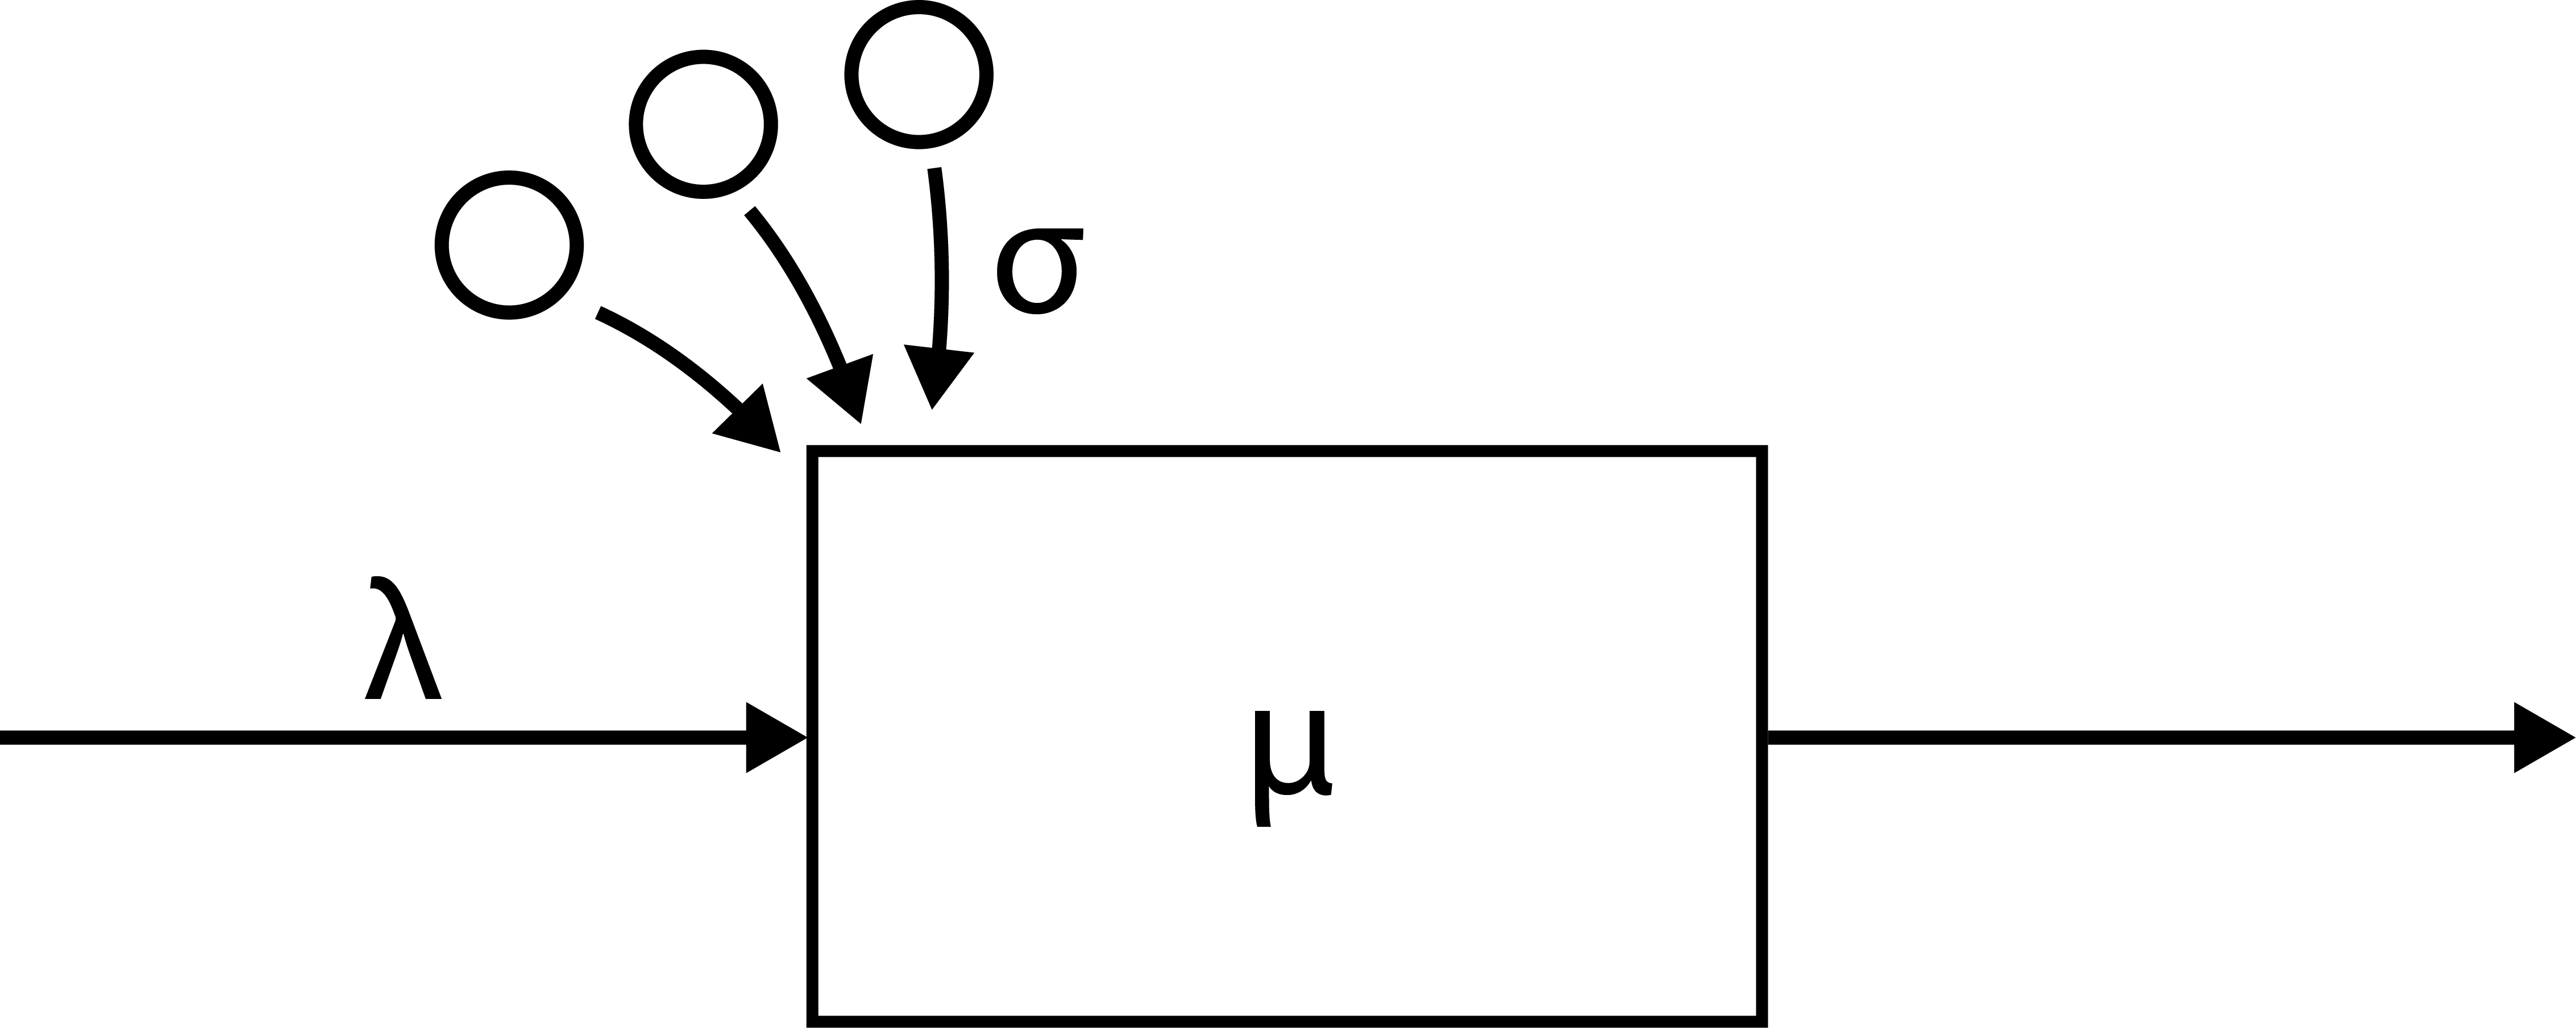
\includegraphics[scale=1,width=\textwidth]{1_sim_example.png}
	\caption{Пример системы ТМО}
	\label{sys_tmo_example}
\end{figure}

Алгоритм моделирования функционирования представленной системы массового обслуживания при помощи очереди событий представлен ниже.
Введем следующие обозначения:
\begin{enumerate}
	\item $Q$ --- очередь, хранящая моменты наступления предстоящих событий в системе и функционирующая по принципу кучи, когда извлекаемый элемент является минимальным среди содержащихся в ней;
	\item $T_{curr}$ --- текущее время моделирования;
	\item $T_{end}$ --- момент окончания моделирования;
	\item $t_i$ --- момент наступления события $i$ в системе. 
	\end{enumerate}

\begin{figure}[H]
	\centering
	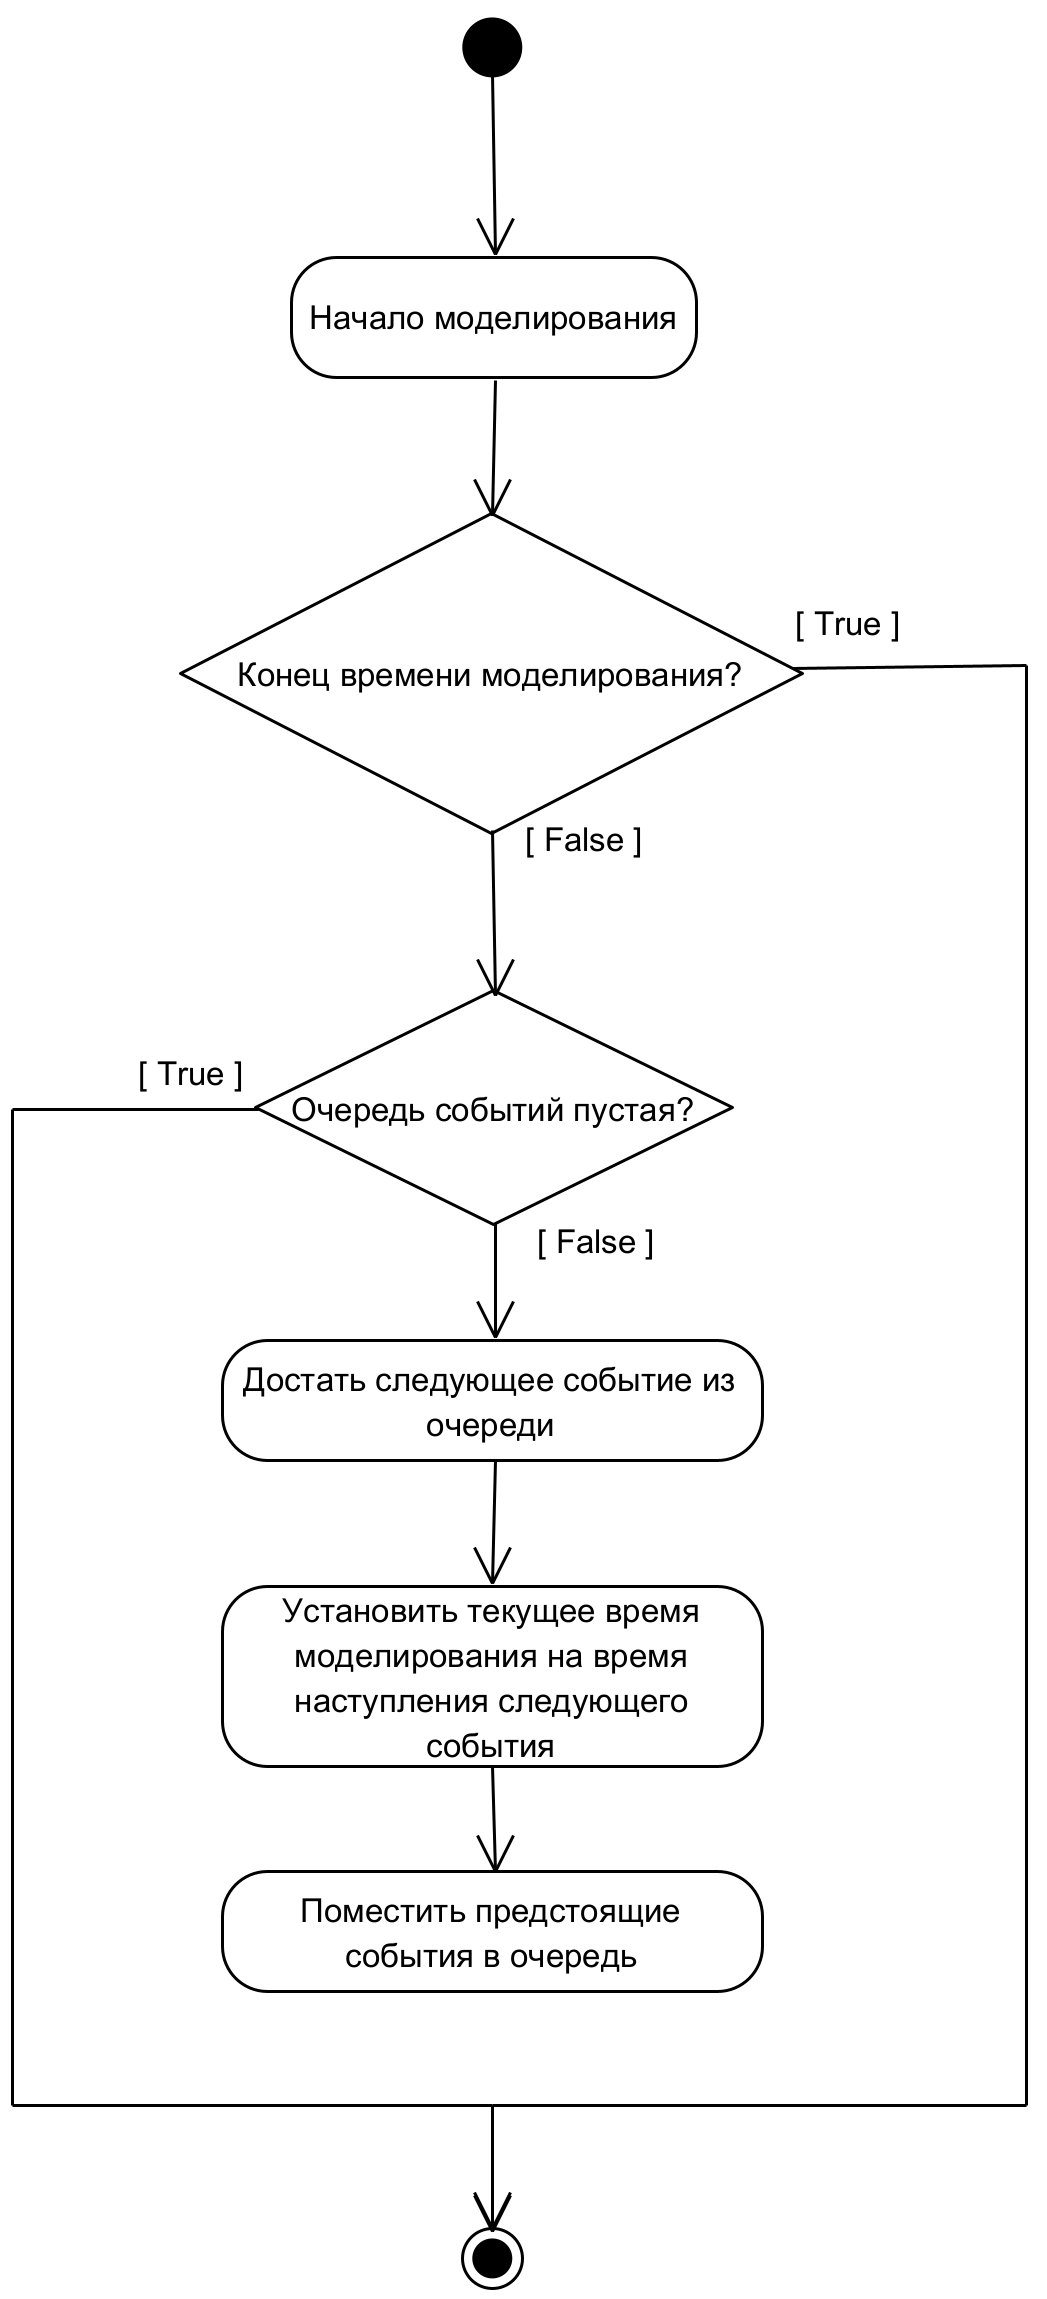
\includegraphics[scale=0.35]{sim_algo.png}
	\caption{Алгоритм моделирования}
	\label{sys_tmo_algo}
\end{figure}

Так, при каждой итерации моделирования из $Q$ достается момент наступления следующего события $t_i$, в свою очередь текущее время моделирования устанавливается как $T_{curr} = t_i$. Наступление события $i$ позволит получить время наступления последующего события $t_j$ (например, заявка успешно поступила на прибор из входящего потока в момент $t_i$, и $t_j$ будет являться момент окончания ее обслуживания), которое поместить в $Q$ и итерация алгоритма завершится, и процесс будет повторятся, пока $Q$ опустеет, либо $T_{curr} = T_{end}$.

Однако для получения достоверных результатов при помощи имитационного моделирования требуется достаточный объем выборки данных, получаемый при работе алгоритма \cite{лобач2004имитационное,моисеев2016исследование}. Определение требуемого объема выборки является отдельной подготовительной задачей и может решаться эмпирически путем подбора такого количества итераций алгоритма, при котором погрешность моделирования, выражаемая, к примеру, среднеквадратическим отклонением \cite{алиев2013погрешности}, становится несущественной.

Так как моделирование подразумевает сравнение получаемой выборки, в частности законов ее распределения, для проверки некой гипотезы о соответствии исследуемой математической модели, также требуется набор критериев и метрик для этого. В общем случае такой метрикой может выступать расстояние Колмогорова, являющимся максимальной по модулю разницей между распределениями вероятностей:
\begin{equation}\label{kdistance}
	\Delta = \underset{0 < i < \infty}{max}\bigg\rvert \sum_{v=0}^{i} (P_0(v) - P_1(v))\bigg\rvert.
\end{equation}
Данная формула также применима для случаев с многомерными распределениями вероятностей \cite{fasano1987multidimensional}. 
\section {Разработка имитационной модели}
В данном разделе описывается процесс проектирования и разработки ключевой составляющей комплекса программ для анализ систем массового обслуживания --- имитационной модели. Проектирование программы начинается с разработки предметной области по предварительно составленным требованиям. В данном случае, делается упор на универсальность модели и возможность встраивания в непосредственный	процесс анализа. Также особое внимание уделяется процедуре проведения численных экспериментов. Численные результаты являются наиболее репрезентативными в случае, если было проведено достаточное количество экспериментов при наборах параметров, которые описывают функционирование модели в различных ситуациях. Такой подход позволяет удостовериться в верности теоретической стороны исследования посредством анализа объемной выборки данных о работе модели.

Предметная область программы была разработана с учетом следующих требований к ее работе и процессу взаимодействия с пользователем. Требования были составлены исходя из имеющегося опыта анализа систем массового обслуживания при помощи имитационного моделирования и опираясь на реализации имеющихся инструментов \cite{yakimov2017comparison}:
\begin{enumerate}
	\item Производительность. Инструмент должен обладать достаточным быстродействием, чтобы в течение адекватного времени проводить имитационное моделирование;
	\item Возможность моделирования широкого спектра моделей теории массового обслуживания, иначе --- универсальность;
	\item Инструмент должен иметь возможность проведения масштабных экспериментов. Другими словами, программа должна быть оптимизирована для запуска большого количества моделей одновременно и параллельно;
	\item Способ задания параметров должен позволять выполнять эксперименты повторно;
	\item Возможность конфигурирования модели. Это означает, что инструмент должен позволять настраивать различные аспекты имитационного моделирования для каждого случая в отдельности;
	\item Возможность производить сбор данных о работе модели в требуемом контексте. Иначе говоря, инструмент должен позволять собрать конкретные статистические данные имитационного моделирования в зависимости от поставленной задачи;
	\item Интеграция в процесс анализа. Другими словами, имитационное моделирование должно быть одним из инструментов среды, в которой проводится анализ. Из данного требования вытекает и выбор целевой программной среды для разработки;
	\item Легкая расширяемость. Исходный код программы должен предоставлять возможность добавления новой логики.
\end{enumerate}

\subsection{Предметная область}
Исходя из выше представленных требований, инструмент должен иметь возможность производить моделирование различных систем массового обслуживания. Исходя из этого, наиболее гибким вариантом реализации данного требования будет включить построение модели в процесс работы с инструментом. Так, у пользователя появляется возможность конструировать требуемую под задачу систему массового обслуживания.

Для достижения предложенного подхода предлагается использовать конструирование блоками \cite{valentin2002simulation} --- инструмент будет включать в себя набор атомарных элементов систем массового обслуживания (обслуживающий прибор, входящий поток и т.д.), которые будут работать по принципу черного ящика, однако связь между элементами и промежуточные этапы будут доступны для конфигурирования. Такой подход позволяет создать абсолютно любую вариацию системы массового обслуживания и используется не только в имитационном моделировании. Зачастую подобное архитектурное решение можно наблюдать в программных комплексах, предназначенных для программирования сложных взаимодействий между объектами. В 3D--графике зачастую используется схожий процесс работы, основанный на графах, где вершины представляют собой алгоритмы и объекты, а ребрами являются взаимодействия между ними. Например, в ПО для создания эффектов и симуляции взаимодействия физических тел Houdini используется именно такой подход \cite{claes2009controlling}.

Принцип работы имитационной модели базируется на обработке событий, происходящих в системе во время ее функционирования. Под событиями понимаются перемещения заявок по элементам системы. Обработка включает в себя регистрацию времени наступления события.

Исходя из вышеперечисленного, для разработки инструмента выбран объектно--ориентированный подход. Его преимуществом является возможность построения абстракций над логикой работы конкретных элементов системы, что позволяет удовлетворить требованию легкой расширяемости и позволить конструирование модели блоками в процессе анализа. 

Объектно--ориентированный подход \cite{fowler1997analysis} к реализации предметной области подразумевает выделение из нее отдельных сущностей, которые могут быть представлены одним самостоятельным объектом, выполняющим конкретную задачу.

Процесс моделирования заключается в перемещении заявок от одного элемента к другому. В очередной условный момент времени $T_{cur}$ местонахождение каждой заявки и ее характеристики могут меняться. По этой причине для каждой заявки вводится условный момент времени моделирования, когда она изменит своё состояние --- $T_{shift}$. В момент времени, когда $T_{shift} = T_{curr}$, заявка перемещается в очередной элемент модели, и  $T_{shift}$ обновляется им в зависимости от заданных параметров.

В первую очередь, как ранее было указано, выделим элемент модели --- объект, который содержит некую вычислительную логику и обрабатывает заявки в соответствии с этой логикой. Пример элемента модели является обслуживающий прибор.

Для того, чтобы соединить элементы в единую модель, потребуется определенном образом указать, как заявки будут перемещаться между элементами. Для этой цели выделим сущность --- маршрутизатор. Однако, в зависимости от реализации элемента, он может иметь разное количество связей, с помощью которых будут перемещаться заявки. Таким образом, требуется ввести сущность, которая регулирует количество и качество возможных соединений элемента --- слот.

Заявка также представлена сущностью.

Поскольку элемент модели работает по принципу черного ящика, то не следует отягощать его логику сбором данным о моделировании. Для этой цели можно использовать маршрутизатор, отслеживая характеристики перемещения заявок в нужных участках модели. Исходя из этого, логику сбора статистики можно вынести в отдельную сущность, что позволит добавить в данный процесс разнообразную логику.

Итак, в предметной области программы были выделены следующие сущности:
\begin{itemize}
	\item Элемент системы --- объект, являющийся частью модели и выполняющий обработку заявок на протяжении ее работы.
	\item Заявка --- объект, перемещающийся по системе и подлежащий обработке.
	\item Маршрутизатор --- объект, образующий односторонний туннель для перемещения заявок от элемента системы к другому.
	\item Слот --- объект, служащий для соединения двух элементов при помощи маршрутизатора.
	\item Сборщик статистики --- объект, собирающий данные о перемещении заявок по маршрутизатору;
	\item Генератор задержки --- служит для генерации случайных величин с требуемым распределением.
\end{itemize}

\subsection{Объектная модель предметной области}
На основе выделенных сущностей и описанного принципа работы программы была построена ее объектная модель, в последствии использованная для реализации.

Для обеспечения универсальности и возможности добавления новых разновидностей элементов модели был введен общий для них интерфейс Producer. Такое решение, в качестве побочного эффекта, также может позволять использовать различные элементы системы в несвойственных для них позициях в модели.
\begin{figure}[H]
	\centering
	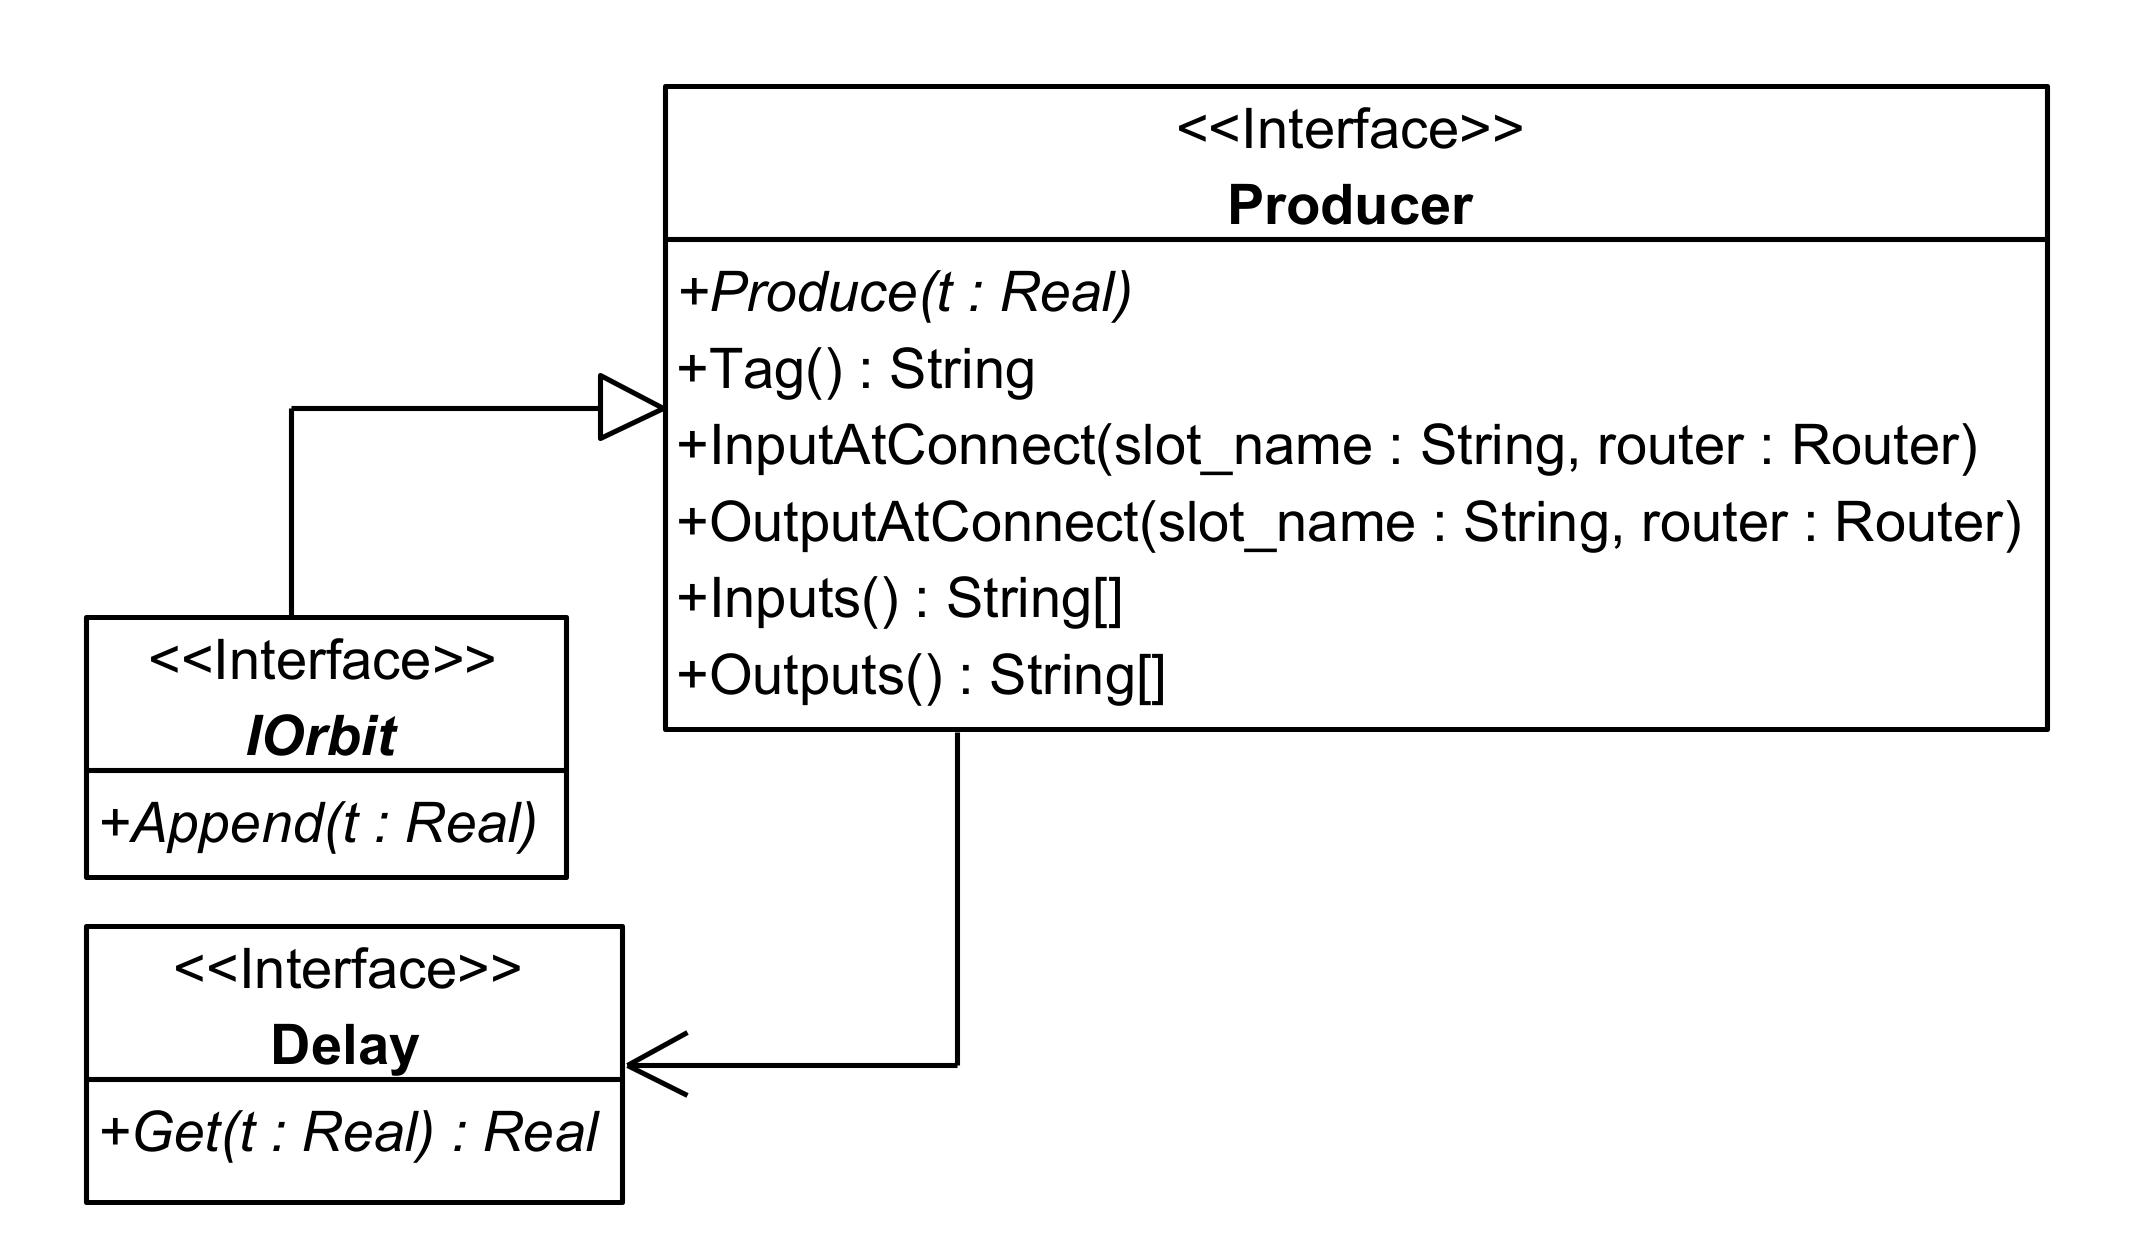
\includegraphics[scale=0.3]{d_producer.png}
	\caption{Интерфейс Producer}
	\label{d_producer}
\end{figure}

В абстрактном методе Produce должна находится логика работы элемента системы, именно этот метод будет вызываться в каждой итерации работы модели, возвращая вектор моментов времени наступления событий в элементе. Также в интерфейсе определены вспомогательные методы Tag, InputAtConnect, OutputAtConnect, Inputs и Outputs, служащие для соединения элементов между собой. Метод Tag возвращает константную строку, определенную для каждой реализации интерфейса Producer. Слоты элемента разделена на два класса --- входящие, которые позволяют принимать элементу заявки, и выходящие, позволяющие ему их отправлять. Методы InputAtConnect и OutputAtConnect позволяют присоединять к маршрутизатору входящие и выходящие слоты соответственно, указывая название слота для соединения. 

Другим важным элементом предметной области является объект, генерирующий время задержки заявок в процессе их перемещения и позволяющий проводить эксперименты, когда элементы системы могут задавать задержку для заявки разного рода. Для этой цели служит интерфейс Delay. Он имеет единственный метод Get, возвращающий сгенерированную случайную величину.
\begin{figure}[H]
	\centering
	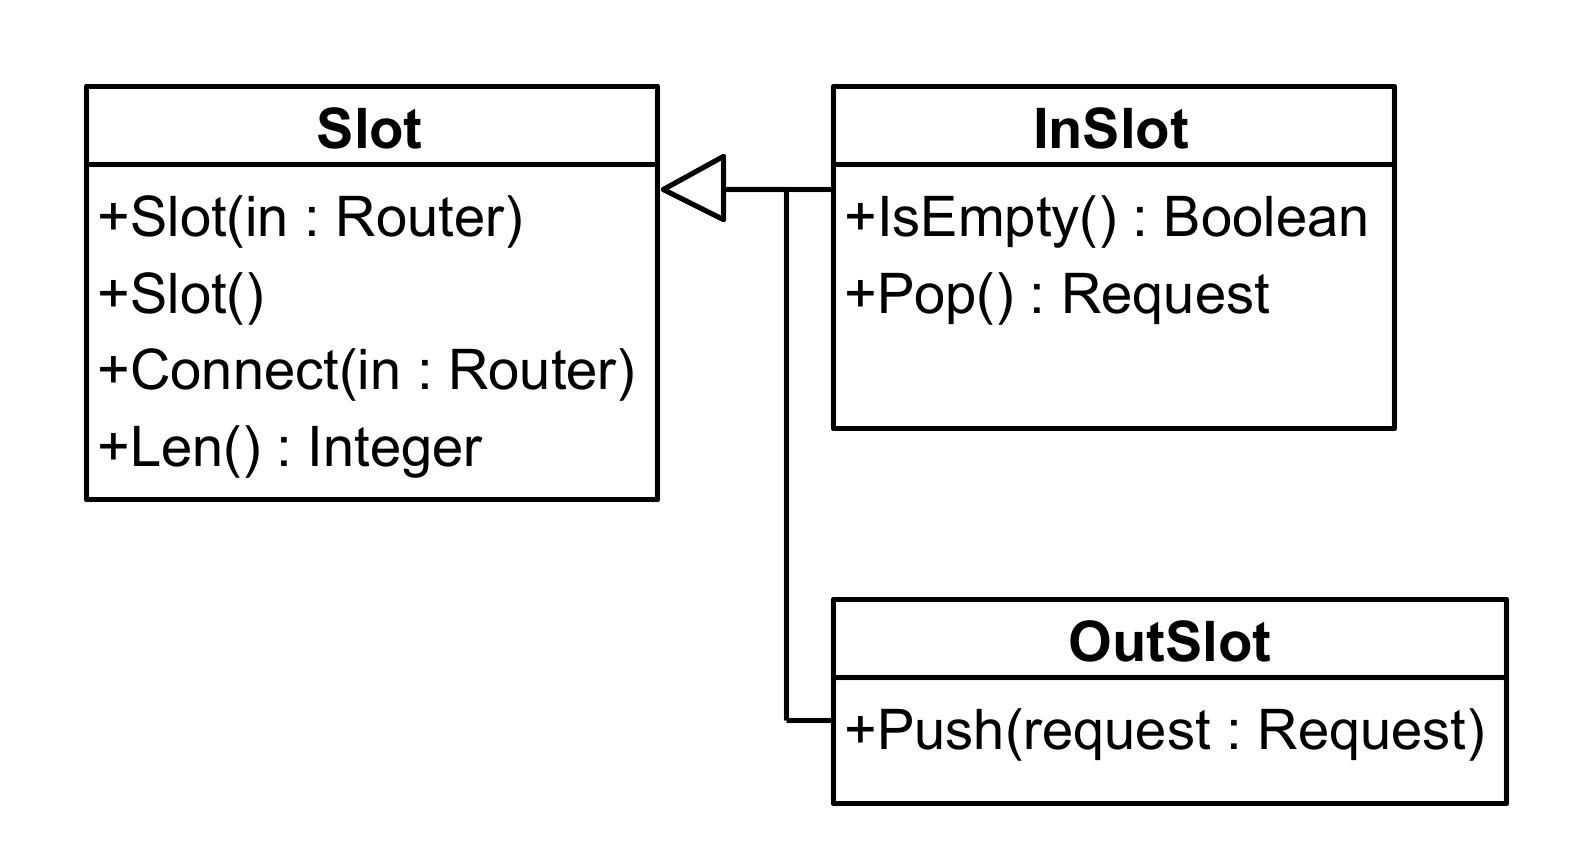
\includegraphics[scale=0.3]{d_slot.png}
	\caption{Класс Slot и его наследники}
	\label{d_slot}
\end{figure}

Слоты используются в элементах системы для задания ограничения на возможные связи между другими элементами. К примеру, входящий поток может иметь только один выход для заявок, которые им генерируются, и не имеет входов, поскольку порождает заявки самостоятельно. В свою очередь, орбита должна иметь один вход для поступающих на нее заявок и один выход для отправления их обратно. Для разграничения логики работы слота на принимающий и отправляющий введено два наследника --- InSlot, способный только принимать заявки при помощи метода Pop и OutSlot, предназначенный лишь для их отправления при помощи метода Push. Среда для переправки заявок между слотами обеспечивается за счет класса Router.

\begin{figure}[H]
	\centering
	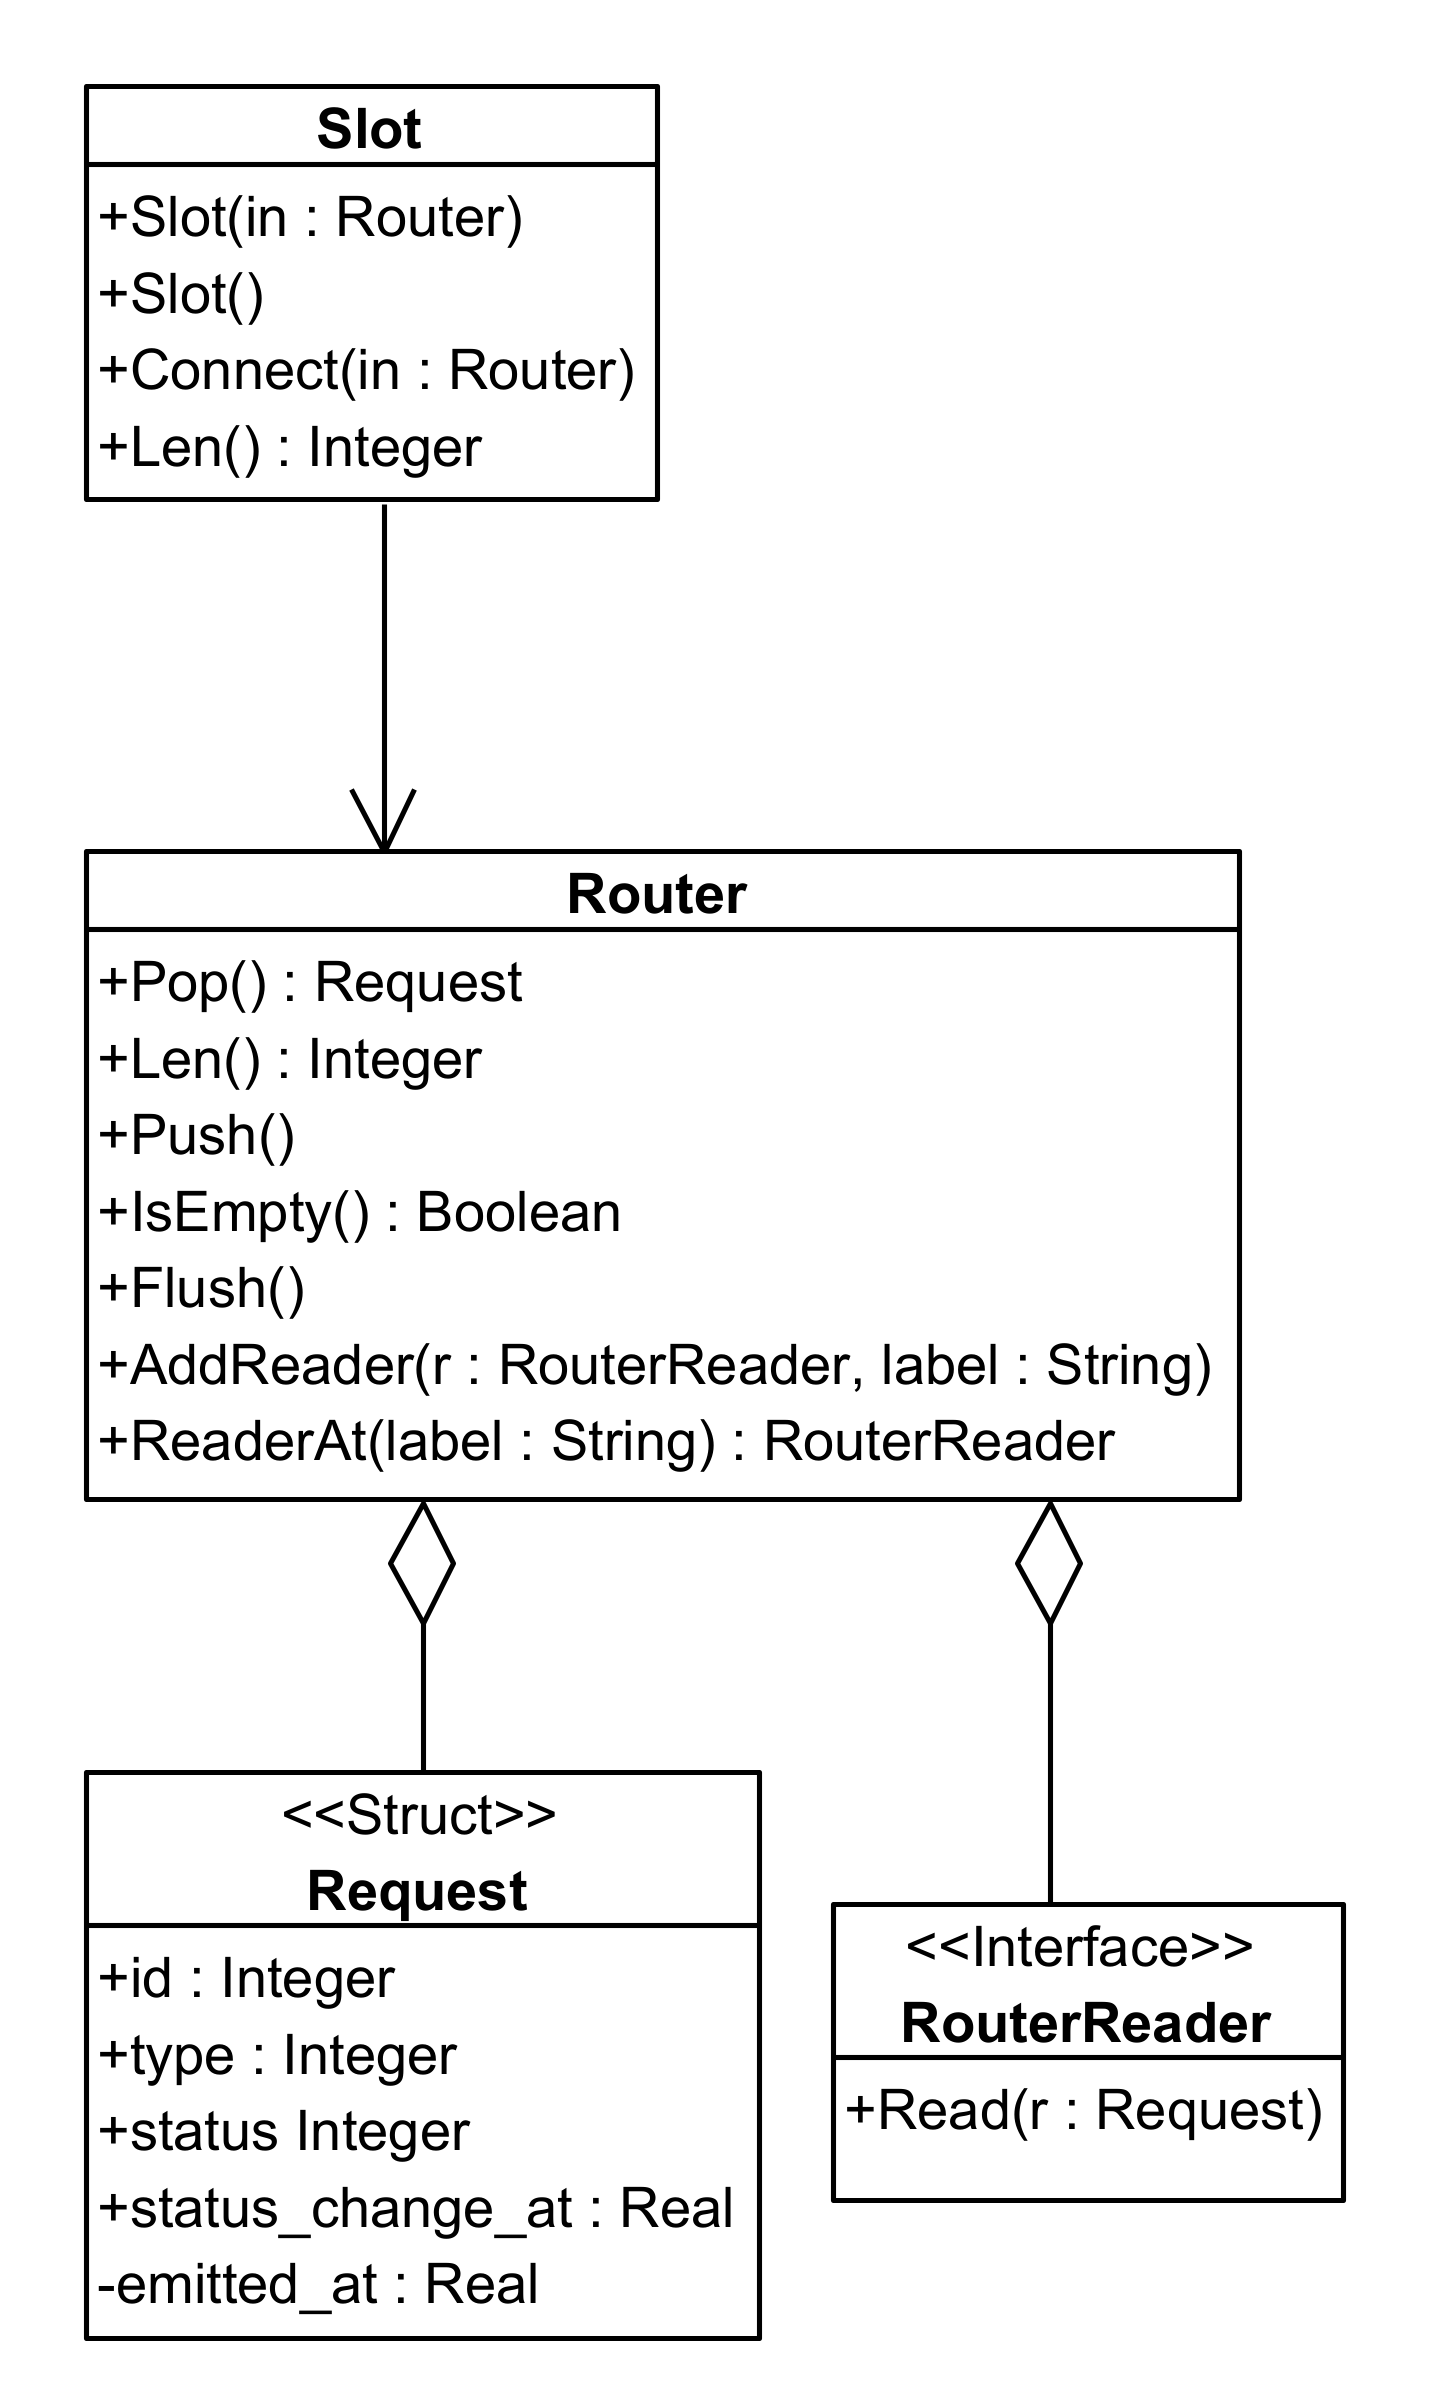
\includegraphics[scale=0.3]{d_router.png}
	\caption{Класс Router}
	\label{d_router}
\end{figure}
Маршрутизатор представляет собой очередь, работающую по принципу FIFO. Таким образом, он позволяет элементам системы взаимодействовать с заявками между итерациями, когда очередная заявка еще ожидает обработки, но текущая итерация подошла к концу. Управление очередью заявок осуществляется при помощи методов Push (поместить заявку в очередь), Pop (достать заявок из очереди), Len (получить текущую длину очереди), IsEmpty (пуста ли очередь). Методы AddReader и ReaderAt предназначены для управления наборов сборщиков статистики. AddReader позволяет добавить новый сборщик статистики под указанным ярлыком, который позволит обращаться к нему в последствии при помощи метода ReaderAt для доступа к собранных данным.

Заявка представлена структурой Request, содержащей момент изменения ее состояния status\_change\_at ($T_{shift}$), тип, служащий для разделения способа происхождения заявки, статус, отражающий этап ее обработки (обслужена, в процессе обслуживания, в пути, покинула систему) и время, когда заявка была создана.

Ниже представлена полная объектная модель предметной области, объединяющая ранее представленные классы и интерфейсы.
\begin{figure}[H]
	\centering
	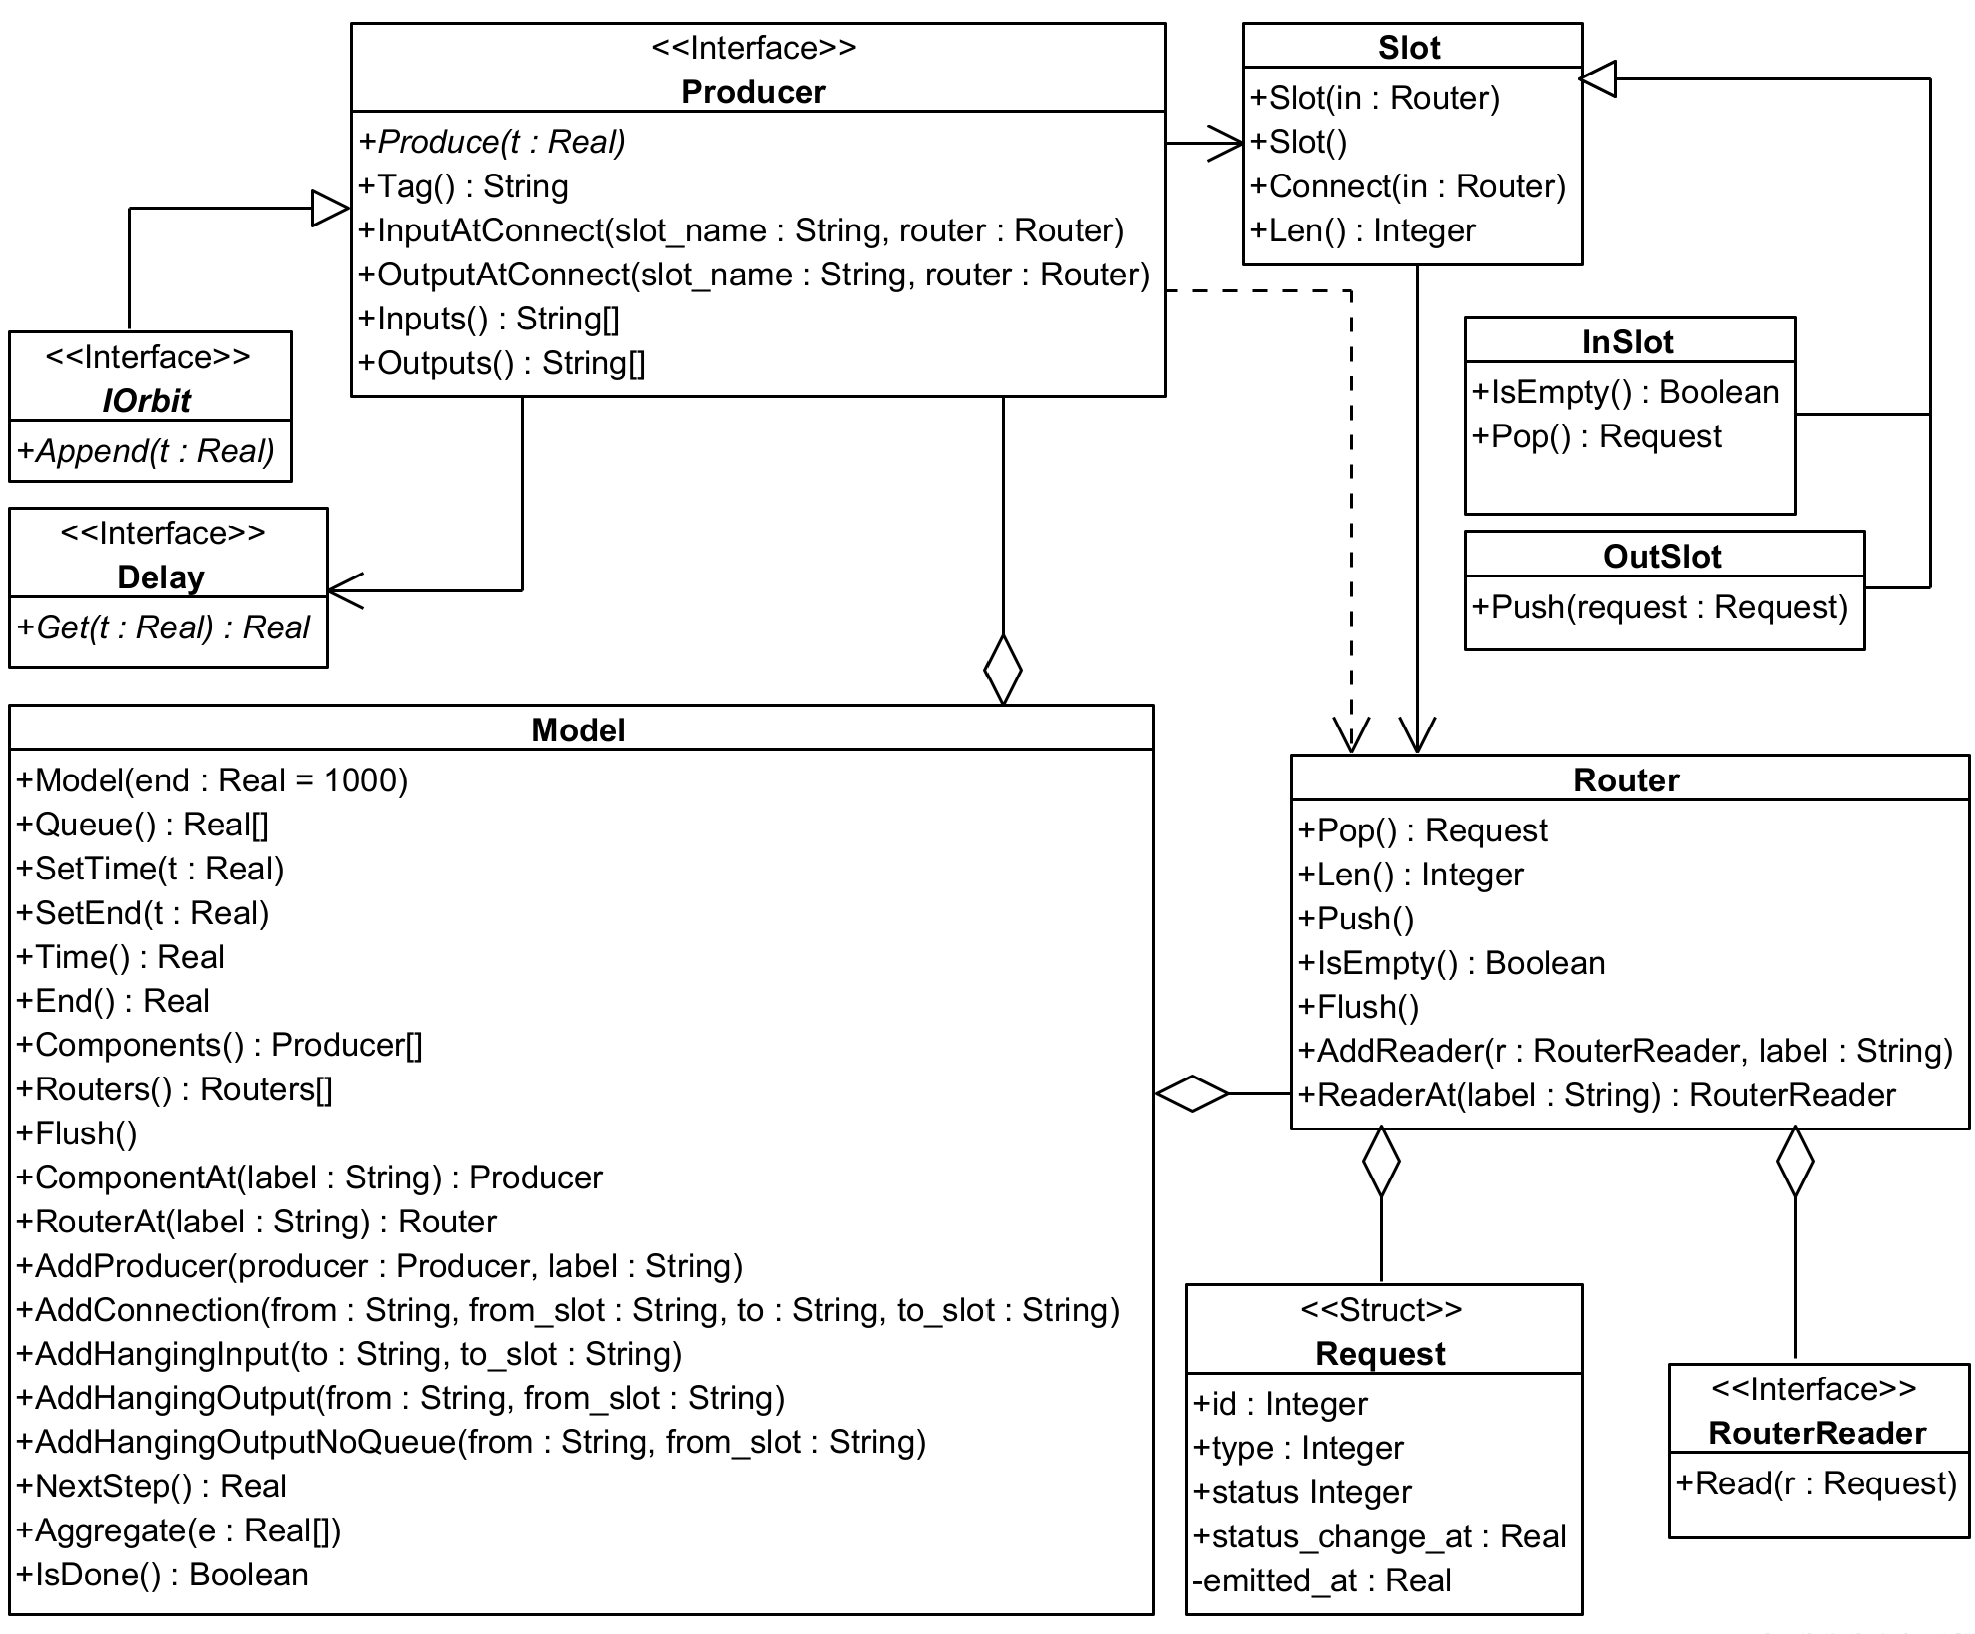
\includegraphics[scale=0.3]{d_d.png}
	\caption{Объектная модель предметной области}
	\label{d_d}
\end{figure}

Как видно на рисунке \ref{d_d}, предметная область содержит специальный агрегирующий класс Model, предназначенный для управления процессом моделирования в рамках одной системы. Он позволяет построить модель при помощи методов AddProducer (добавление нового элемента в модель) и AddConnection(добавление маршрутизатора между существующими элементами). AddConnection имеет три частных случая: AddHangingInput --- добавляет маршрутизатор на входящий слот одного элемента, AddHangingOutput --- добавляет маршрутизатор на выходящий слот элемента, AddHangingOutputNoQueue --- аналогичен AddHangingOutput, но заявки не сохраняются в маршрутизаторе. Три перечисленных метода позволяют вручную отправлять заявки в модель, а также устанавливать поток заявок между отдельными моделями.

Метод Queue возвращает текущий вектор моментов наступления событий в системе. SetTime, Time, SetEnd, End устанавливают либо возвращают текущее условное время и условное время окончания моделирования соответственно. Методы Components и Routers возвращают список имеющихся в модели элементов и маршрутизаторов соответственно. Методы ComponentAt и RouterAt предоставляют доступ к конкретному элементу или маршрутизатору. Метод Aggregate добавляет в вектор предстоящих событий новые, а метод NextStep сдвигает время моделирования на момент наступления ближайшего события и возвращает его. Метод IsDone позволяет узнать, закончилось ли моделирование (текущее время моделирования стало равно времени окончания моделирования).

Иначе содержимое модели можно представить графически следующим образом (рисунок \ref{model_container}):
\begin{figure}[H]
	\centering
	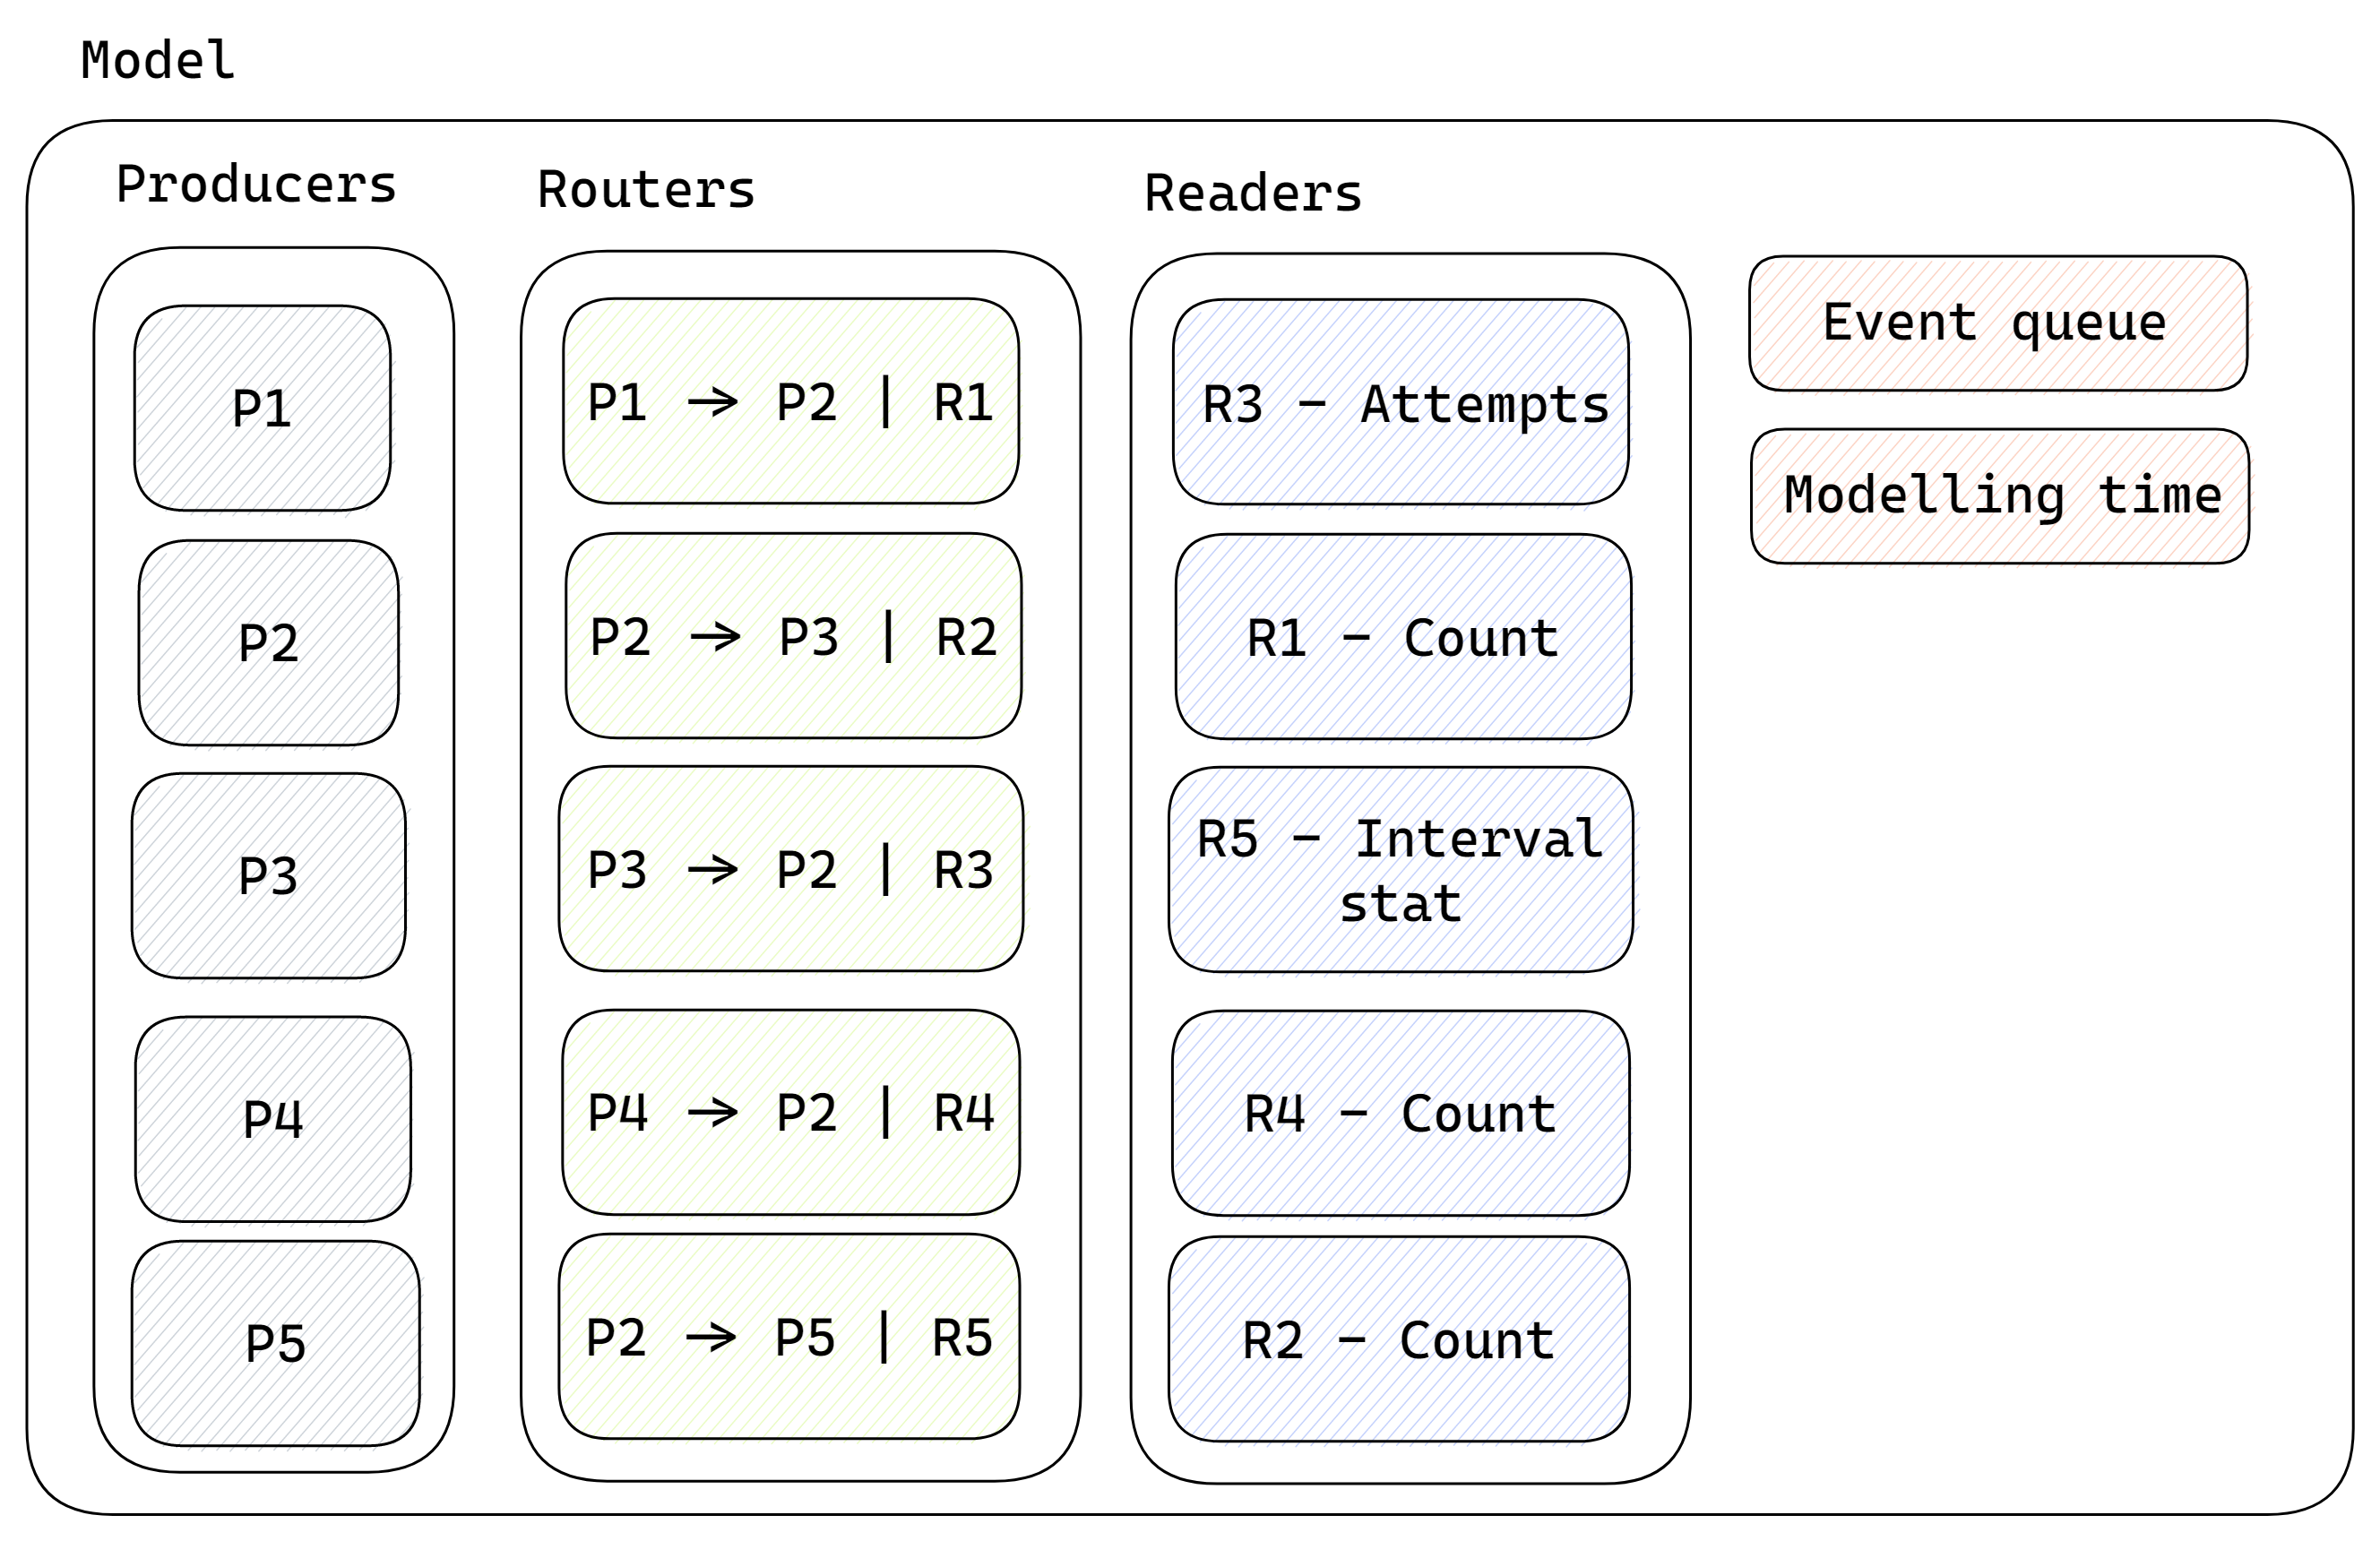
\includegraphics[scale=0.18]{model_container.png}
	\caption{Объектная модель предметной области}
	\label{model_container}
\end{figure}

\subsection{Реализации интерфейсов}
В данном разделе представлены имеющиеся реализации интерфейсов и родительских классов, описанных ранее в предметной области.

Для интерфейса Producer существует три ряда реализаций, разделенных по предназначению согласно теории массового обслуживания. 

Первые классом являются приборы. Среди них:
\begin{enumerate}
	\item SimpleNode --- реализация простейшего обслуживающего прибора, который обслуживает входящие заявки и передает их далее. В случае, если заявка не может получить доступ к прибору, она теряется;
	\item RQNode --- реализация обслуживающего прибора с орбитой. Функционирует аналогично простейшему прибору, однако заявки, не сумевшие попасть на прибор перемещаются на орбиту, откуда снова пытаются захватить его;
	\item RQTNode --- аналогичен прибору с орбитой, но обслуживает два типа заявок: входящие и приходящие из источника повторных вызовов.
\end{enumerate}


Далее описаны источники заявок --- объекты, имеющие только выход для порожденных заявок:
\begin{enumerate}
	\item SimpleInput --- реализация простейшего потока;
	\item MMPPInput --- реализация MAP--потока, имеющего управляющую цепь, которая определяет состояние процесса, в соответствии с которым меняется и интенсивность порождения заявок.
\end{enumerate}

Для орбиты имеется лишь одна реализация.

Отметим, что каждая из реализаций имеет в качестве параметра генераторы случайных задержек, что позволяет существенно менять характеристики функционирования элемента. Для этого интерфейса (Delay) имеются следующие реализации:
\begin{enumerate}
	\item ExponentialDelay --- генератор экспоненциально распределенного времени задержки;
	\item UniformDelay --- генератор равномерно распределенного времени задержки;
	\item GammaDelay --- генератор задержки, имеющей гамма распределение;
 	\item WeibullDelay --- генератор задержки, имеющей распределение Вейбулла \cite{hallinan1993review};
 	\item LognormalDelay --- генератор задержки, имеющей логнормальное распределение.
\end{enumerate}

Для маршрутизатора, помимо основной реализации, имеются два особых случая:
\begin{enumerate}
	\item NoneRouter --- очередь всегда пуста, а заявки, попадающие в нее, уничтожаются. Данный класс предназначен для тех случаев, когда в заявки надо направить в тупик после обслуживания и их учет не требуется;
	\item OutputRouter --- отличается от NoneRouter тем, что учет проходящих по очереди заявок ведется, однако они по-прежнему не хранятся.
\end{enumerate}

Сборщики статистики:
\begin{enumerate}
	\item IntervalRouterReader --- сборщик статистики, предназначенный для получения распределения вероятностей числа прошедших через маршрутизатор заявок разного типа. Класс имеет методы для получения суммарного распределения, среднего, среднеквадратического отклонения и другие;
	\item AttemptCounter --- сборщик, учитывающий количество раз, которое каждая заявка прошла через маршрутизатор, а также суммарное время, потраченное на перемещение до цели;
	\item TimeCounter --- сборщик, учитывающий моменты времени, когда заявки проходили через маршрутизатор.
\end{enumerate}

\subsection{Особенности реализации}
В данном разделе описаны подробности реализации имитационной модели.

 Исходный код, реализующий предметную область, выполнен на языке программирования C++ стандарта 2017 года (C++1z). Выбор в сторону C++ был сделан исходя из требований к инструменту, которые включают производительность и возможность интеграции непосредственно в процесс исследования, о чем подробнее изложено ниже. C++ отлично подходит для написания производительного программного обеспечения, а также обеспечивает гибкость в плане архитектурных решений и управления памятью. Помимо этого С++ является объектно--ориентированным языком программирования, что важно для реализации предметной области. Однако с некоторыми различиями, такими, как отсутствие интерфейсов в явном виде. Вместо них C++ поддерживает абстрактные классы с чистыми виртуальными функциями \cite{schmid2012c++}.
 Помимо этого важными аспектами являются:
 \begin{enumerate}
 	\item Ручное управление памятью. С одной стороны, необходимость разработчику постоянно следить за выделяемой памятью и разрушением экземпляров объектов является недостатком, так как осложняет процесс разработки и способствует возникновению ошибок в управлении памятью, с другой --- дает возможность организовать подходящий под задачу процесс выделения памяти.
 	\item Компиляция. Компилируемые языки всегда превосходят в производительности интерпретируемые, поскольку проверка типов, предупреждение возникших исключений и других ошибок происходят на этапе компиляции, а не в процессе работы программы.
 	\item Статическая типизация. Заранее известные типы объектов ускоряют как компиляцию, так и работу программы ввиду отсутствия проверки типов.
 	\item Объявление без инициализации. C++ позволяет объявить переменную, не инициализируя ее некоторым значением, что экономит время работы.
 \end{enumerate}

 Для сборки программы использовался компилятор GCC \cite{gcc}, поскольку он поддерживается всеми платформами, а также имеет широкий спектр параметров для оптимизации кода на этапе компиляции \cite{branco2015impact}. 
 
 \subsection{Реализация программы в качестве программного пакета для Python}
 Ключевой особенностью реализуемого ПО является возможности работы с ним в среде, где проводится остальные операции по исследованию и анализу системы массового обслуживания. По этой причине инструмент является программным пакетом (библиотекой) для языка Python. Данный язык крайне удобен и популярен для проведения статистического анализа, машинного обучения и других научных исследований, а имеющая оболочка для интерактивной работы IPython позволяет объединить все аспекты работы в общей среде исполнения.
 
 Python реализован на C++, что позволяет разрабатывать к нему расширительные пакеты не только на самом языке, но и на языке реализации, что дает преимущество в производительности и вариативность. Примером подобного пакета, является фундаментальная библиотека для вычислений линейной алгебры и работы с матрицами NumPy, которая лежит в основе многих других пакетов и написана на С++ \cite{numpy}.
 
 Исходный код, относящийся к предметной области строго изолирован, чтобы предоставить максимальную расширяемость имеющихся интерфейсов. За привязку исходного кода с библиотеке Python отвечает библиотека Pybind11 \cite{pybind}. Она позволяет скомпилировать код, написанный на языке C++ в пакет для Python, при этом код изначально может быть изначальное не предзначен для этого. Таким образом, становится возможным строго разделить интерфейс, с которым взаимодействует пользователь и внутреннюю логику работы программы.
 
 Ниже приведен пример привязки исходного кода класса Router. Тело методов опущено для лучшей читаемости.
 
 Код на C++:
 \lstset{language=C++,
 	basicstyle=\linespread{0.8}\ttfamily,
 	caption={Исходный код класса Router},
 	label={router_listing}
 }
 \begin{lstlisting}
 class Router
 {
 	public:
 	std::vector<Request> q;
 	std::unordered_map<std::string, RouterReader &> readers;
 	friend class InSlot;
 	friend class OutSlot;
 	friend class Slot;
 	
 	Router()
 	void AddReader(RouterReader &r, std::string label)
 	std::unordered_map<std::string, RouterReader &> &Readers()
 	RouterReader &ReaderAt(std::string label)
 	virtual Request Pop()
 	virtual int Len()
 	virtual void Push(Request request)
 	virtual bool IsEmpty()	
 	virtual void Flush()
 };
 \end{lstlisting}

Как видно из листинга \ref{router_listing}, маршрутизатор содержит очередь q, словарь ссылок на сборщиков статистики readers, а также объявления о дружественных классах для семейства классов Slot, поскольку они тесно связаны между собой. Ниже представлена привязка данного класса при помощи Pybind11, позволяющая инстанциировать объекты в интерпретаторе Python и работать с ними, но управление памятью и вызов функций будет происходить на стороне C++. Другими словами, с помощью такого подхода создается оболочка для реализации предметной области программы на C++:

\lstset{language=C++,
	basicstyle=\linespread{0.8}\ttfamily,
	caption={Привязка класса Router при помощи Pybind11},
	label={py_router_listing}
}
\begin{lstlisting}
	py::class_<Router>(m, "Router", "Request queue")
	.def(py::init())
	.def("len", &Router::Len, "Returns number of requests contained")
	.def("push", &Router::Push, "request"_a, "Push request in queue")
	.def("pop", &Router::Pop, "Pop request from queue")
	.def("is_empty", &Router::IsEmpty, "Check if queue is empty")
	.def("flush", &Router::Flush, "Clears router queue")
	.def("add_reader", &Router::AddReader, "reader"_a, "label"_a, py::keep_alive<1, 2>(), "Add request reader")
	.def("readers", &Router::Readers, py::return_value_policy::reference, "dictionary of readers")
	.def("reader_at", &Router::ReaderAt, py::keep_alive<1, 0>(), py::return_value_policy::reference, "get reader")
	.def_readonly("pushed_count", &Router::pushed_count, "number of pushed requests")
	.def_readonly("popped_count", &Router::popped_count, "number of popped requests")
	.def_readwrite("__readers__", &Router::readers)
	.def_readonly("__q__", &Router::q);
\end{lstlisting}

Так, Pybind11 позволяет переименовать сигнатуры функций, в частности, указать новые названия методов, аргументов, а также указать пояснение для документации к каждому методу и классу. То же самое возможно сделать для всего модуля в целом, что позволить совместить его в одном пакете с имеющимся кодом на Python, либо создать вокруг нее еще один слой интерфейса:
\lstset{language=C++,
	basicstyle=\linespread{0.8}\ttfamily,
	caption={Объявление модуля Pybind11},
	label={py_module_listing}
}
\begin{lstlisting}
PYBIND11_MODULE(simulation, m)
{
	m.attr("__name__") = "q_analysis.simulation";
	m.doc() = "Python library for retrial queuing system modeling";
	...
}
\end{lstlisting}

 Помимо этого, важно отметить, что при привязке требуется указать, как именно будет происходить распоряжение памятью при создании и удалении объектов. В Python все переменные являются указателями, которые содержать в себе счетчик ссылок, означающий количество ссылающихся указателей на область в памяти. Как только счетчик становится равным нулю, объект уничтожается интерпретатором, что может повлечь за собой различного рода ошибки доступа к памяти и ее утечку. Во избежание перечисленных ошибок Pybind11 позволяет указать время жизни объекта, являющегося аргументом и возвращаемым значением по принципу Nurse--Patient:
 
 \lstset{language=C++,
 	basicstyle=\linespread{0.8}\ttfamily,
 	caption={Указание времени жизни объекта и тип возращаемого значения в Pybind11},
 	label={py_router_keep_alive_listing}
 }
 \begin{lstlisting}
 	py::class_<Router>(m, "Router", "Request queue")
 	.def("add_reader", &Router::AddReader, "reader"_a, "label"_a, py::keep_alive<1, 2>(), "Add request reader")
 	.def("reader_at", &Router::ReaderAt, py::keep_alive<1, 0>(), py::return_value_policy::reference, "get reader")
 \end{lstlisting}

В листинге \ref{py_router_keep_alive_listing} для метода add\_reader указано выражение py::keep\_alive<1, 2>(), что означает следующее: аргумент метода reader (индекс 2) не должен удалятся, пока не удален вызывающий метод объект (индекс 1). Данное выражение предотвратит ситуацию, когда аргумент reader может быть удален из памяти еще до того, как попадет в функцию add\_reader. Иными словами, выражение keep\_alive<$i,j$> указывает, что объект $j$ должен прожить хотя бы столько же, сколько проживет объект $i$. Индексом, равным единице, всегда является вызывающий объект; последующие индексы относятся к аргументам; индекс, равный нулю, означает возвращаемое значение функции. Пример использования указания времени жизни возвращаемого значения можно наблюдать в привязке метода reader\_at: поскольку данный метод является аналогом оператора индексации, крайне важно, чтобы ссылка на объект, возвращаемая методом не была удалена при обращении. Также для этого же метода указана политика возвращаемого значения --- reference. Это означает, что при возращении значения из функции управление данным объектом не переходит к Python, и ответственным за своевременное удаление объекта из памяти является код на стороне C++.

\subsection{Интеграция в процесс исследования}
После успешной компиляции проекта, становится возможным использовать программу как нативный пакет Python, что и позволяет встроить программу непосредственно в среду, где проводится исследования. В свою очередь процесс работы был вдохновлен известной библиотекой для машинного обучения PyTorch \cite{pytorch}, где модель, в данном случае нейронная сеть, предварительно составляется из набора слоев требуемой конфигурации и уже в последствии обучается. Попытка использовать подобный принципе была сделана и в случае имитационной модели: 
 \lstset{language=Python,
	basicstyle=\linespread{0.8}\ttfamily,
	caption={Указание времени жизни объекта и тип возращаемого значения в Pybind11},
	label={python_example}
}
\begin{pyin} [pyexampleinit]
from q_analysis import simulation as q
model = rq.Model()
model.set_time(0) 
model.set_end(1000000)
\end{pyin}

\begin{pyin}[pyexampleaddproducers]
model.add_producer(rq.SimpleInput(rq.ExponentialDelay(1.1),0,0),"input")
model.add_producer(rq.SimpleInput(rq.ExponentialDelay(0.6),1,0),"call")
model.add_producer(rq.Orbit(rq.ExponentialDelay(0.81)),"orbit")
model.add_producer(
             rq.RqtNode(rq.ExponentialDelay(1.3),
             rq.ExponentialDelay(1)),"node")
\end{pyin}

\begin{pyin}[pyexampleaddconnections]
nodein = model.add_connection("input","out_slot","node","in_slot")
model.add_connection("call","out_slot","node","call_slot")
model.add_connection("orbit","out_slot","node","orbit_slot")
output = model.add_hanging_output_noqueue("node","out_slot")
model.add_connection("node","orbit_append_slot","orbit","in_slot")
\end{pyin}

\begin{pyin}[pyexampleaddreaders]
model.router_at(output).add_reader(rq.TimeCounter(),"count")
\end{pyin}

В ячейке \ref{pyexampleinit} производится создание модели и задание времени моделирования. Далее, в ячейке \ref{pyexampleaddproducers}, производится добавление элементов в модель:
\begin{itemize}
\item простейший поток с экспоненциально распределенными моментами порождения заявок, интенсивностью $1.1$ и меткой \textquote{input};
\item простейший поток с экспоненциально распределенными моментами порождения заявок, интенсивностью $0.6$ и меткой \textquote{call} в качестве источника вызываемых заявок;
\item орбита с интенсивностью повторного обращения заявок $0.81$ и меткой \textquote{orbit};
\item обслуживающий прибор с повторными обращениями и обратной связью, обрабатывающий входящие заявки в течение экспоненциально распределенной задержки с интенсивностью $1.3$ и вызываемые заявки в течение экспоненциально распределенной задержки с интенсивностью $1$. Имеет метку \textquote{node}.
\end{itemize}

В ячейке \ref{pyexampleaddconnections} производится маршрутизация заявок между элементами модели:
\begin{itemize}
	\item заявки из входящего потока \textquote{input} попадают на прибор \textquote{node};
	\item заявки из источника вызываемых заявок \textquote{call} попадают на прибор \textquote{node};
	\item заявки, находящиеся на орбите \textquote{orbit} пытаются попасть обратно на прибор \textquote{node};
	\item заявки, не сумевшие захватить прибор \textquote{node} отправляются на орбиту \textquote{orbit};
	\item заявки, успешно обработанные прибором \textquote{node} отправляются в тупик.
\end{itemize}

В ячейке \ref{pyexampleaddreaders} к маршрутизатору, который представлен как тупик для обслуженных заявок, добавляется сборщик моментов прохождения заявок через маршрутизатор \textquote{count}. После этого модель готова к запуску и графически может быть представлена как на изображено на рисунке \ref{py_example_model}.

\begin{figure}[H]
	\centering
	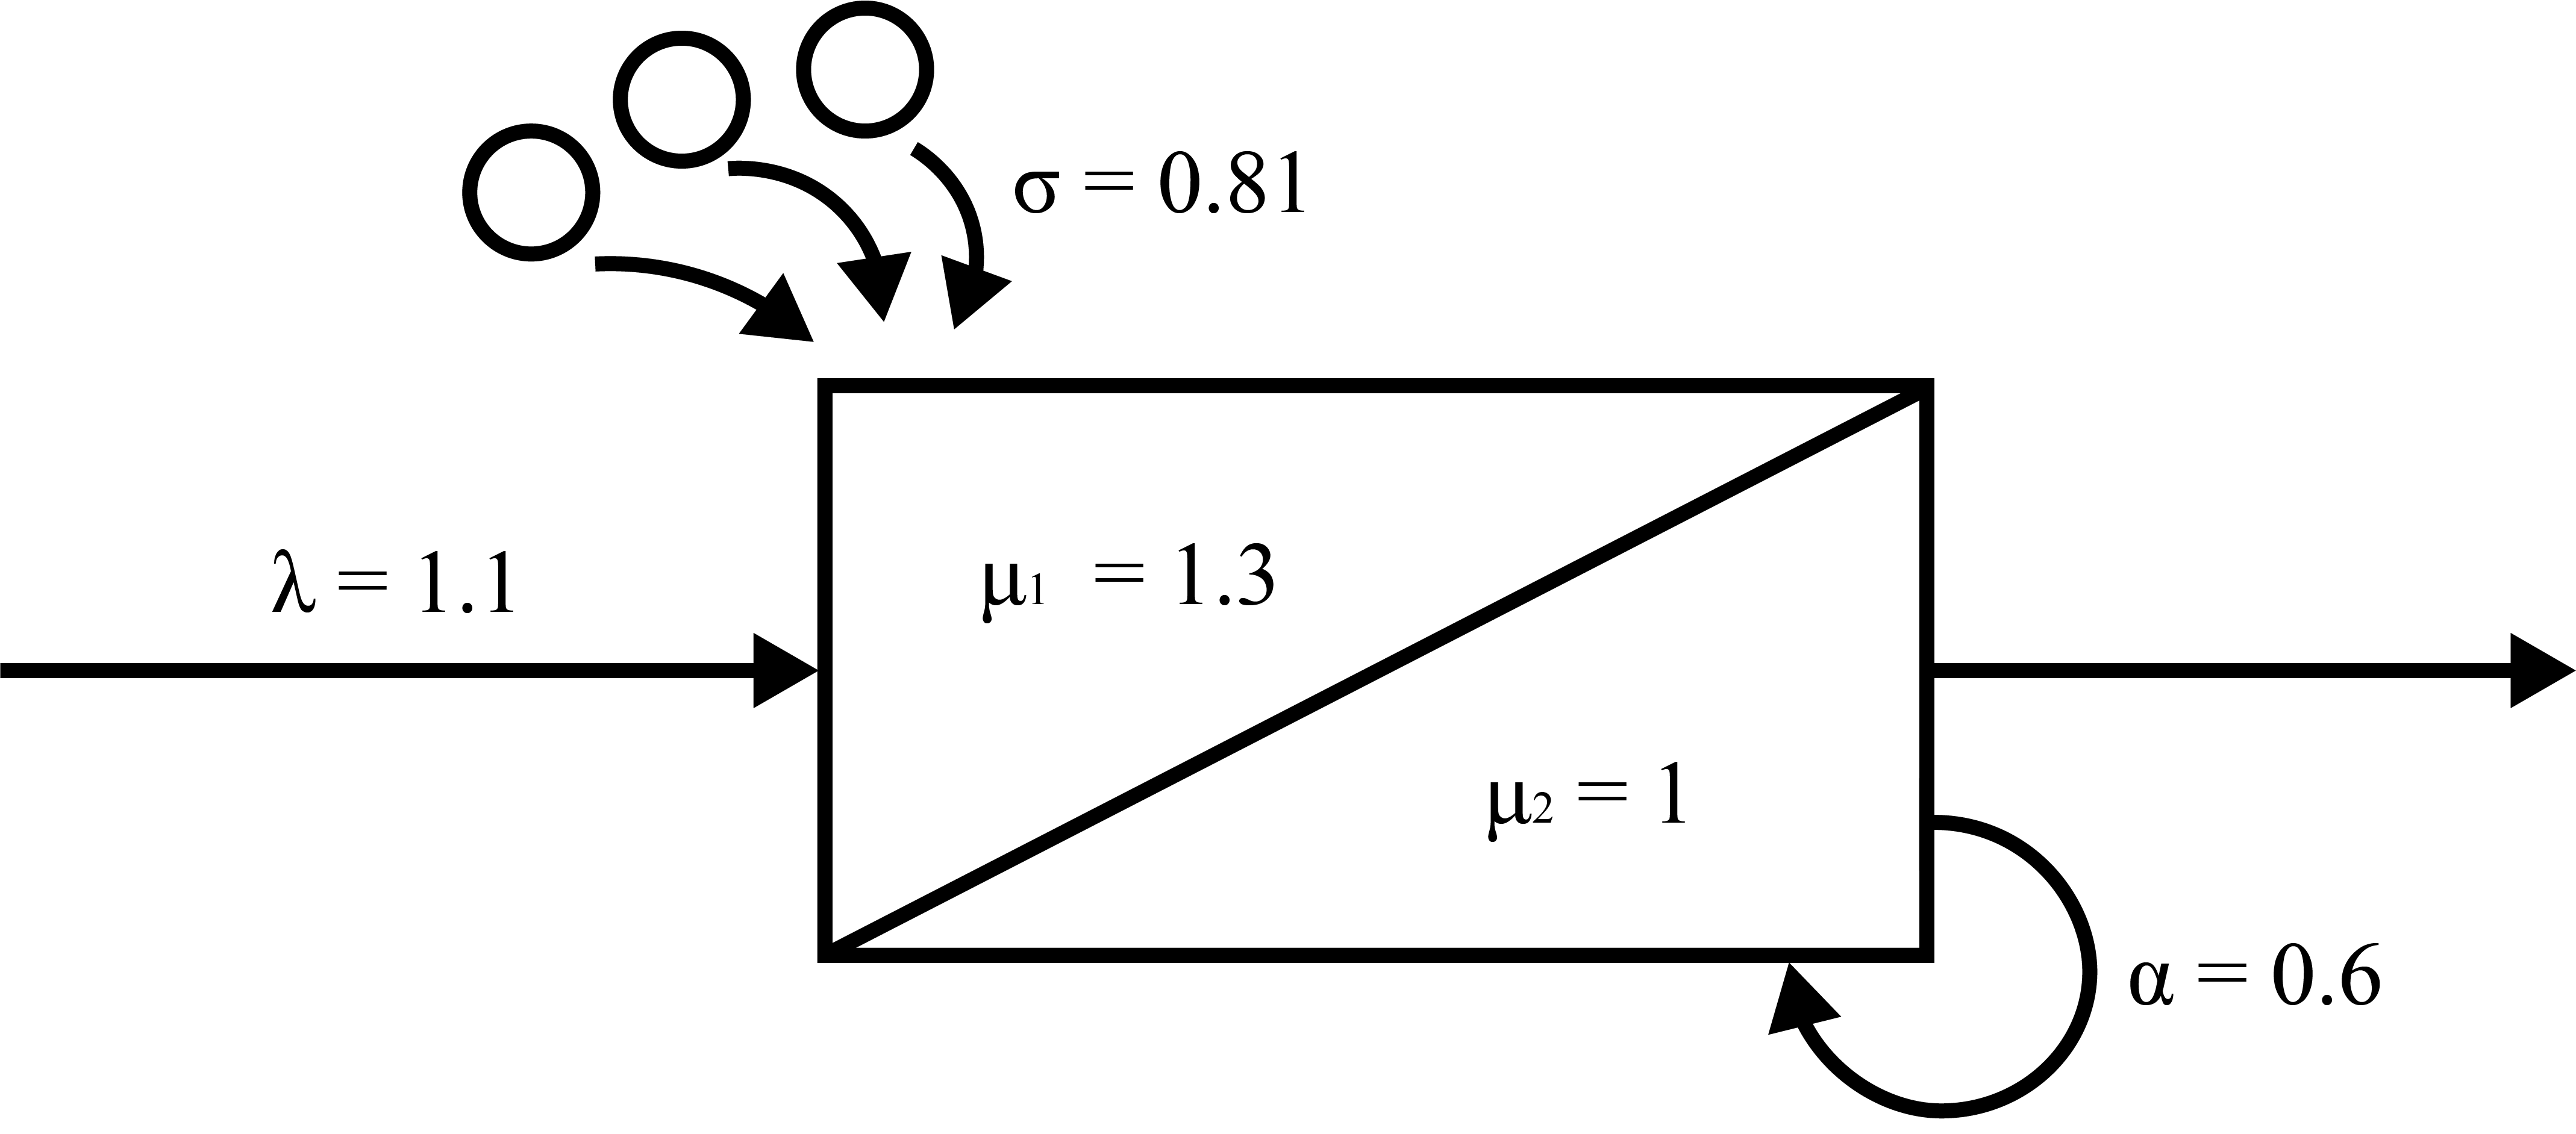
\includegraphics[scale=0.45]{2_sim_example.png}
	\caption{Пример составленной модели}
	\label{py_example_model}
\end{figure}
 
\clearpage 
\section {Вычисление асимптотических результатов}
Имитационное моделирование позволяет нам получать большое количество информации о работе системы, и во многих задачах оно используется для определения области применимости асимптотических результатов. В зависимости от задачи они могут быть получены и вычисляться легко, но в других случаях они могут быть представлены в виде характеристической функции, а для анализа проводится поточечное сравнение распределений вероятности исследуемой характеристики системы. Такая функция может содержать трудно поддающиеся вычислению элементы, среди которых находятся интегралы, матричные экспоненты и др., поскольку получена она была при помощи математического аппарата без первостепенной задачи оптимизации ее вычисления. И на этапе, когда требуется получить значения такой функции, процесс оказывается длительным и трудоемким, так как переход от характеристической функции к распределению вероятностей производится при помощи обратного преобразования Фурье, использующего интегрирование. В ситуации, когда характеристическая функция имеет два, три и более аргументов, вычислительная сложность возрастает во много раз в виду вложенных интегралов. К проблеме трудоемкости также добавляется надобность производить большое количество вычислений, например, для пятисот запусков имитационной модели, результатом которых будет являться двумерное распределение вероятностей размерностью 10 на 10 точек, потребуется 500 раз вычислить то же самое распределение посредством аналитических формул.

В данном разделе предлагается использовать теорию Фурье-анализа сигналов для обращения характеристических функций дискретных распределений. Идея заключается в применении принципов теоремы Котельникова \cite{ястребов2012дискретизация,kuznecov2008} для дискретизации характеристических функций и применения дискретного преобразования Фурье, которое вместо интегрирования использует суммирование и умножение, что гораздо эффективнее. В рамках разрабатываемого программного комплекса этот подход также применяется для обращения характеристической функции и упрощения вычислений, связанных с этим процессов. Данное решение может быть использовано как для анализа систем массового обслуживания, так и в других разделах теории вероятностей, где требуются множественные вычисления.

Как известно, любая случайная величина может быть однозначно определена функцией распределения вероятностей или характеристической функцией \cite{gnedenko2010}. При этом характеристическая функция может быть определена для любой случайной величины (дискретной или непрерывной).

Объектом исследования теории массового обслуживания являются случайные величины и случайные процессы, которые могут быть как непрерывными (например, время ожидания заявки до начала обслуживания, период занятости системы, объем занятого ресурса), так и дискретными (например, число заявок в очереди, число событий, наступивших в потоке за некоторый промежуток времени, число занятых каналов обслуживания). При этом эти величины по своей природе принимают в основном неотрицательные значения.

Для неотрицательных случайных величин характеристическая функция является частным случаем преобразования Лапласа-Стилтьеса от функции распределения вероятностей с мнимым аргументом. Соответственно, характеристическая функция обладает свойствами преобразования Лапласа-Стилтьеса. С другой стороны, в общем случае взаимное соответствие характеристической функции и функции распределения вероятностей соответствует теории Фурье-анализа, безусловным преимуществом которого является свойство двойственности, то есть схожесть переходов от одной функции к другой. Это позволяет, решая задачу для характеристических функций, впоследствии по явным интегральным формулам переходить к функциям распределения.

Для дискретных распределений принято использовать не характеристическую функцию, а производящую \cite{kalinina2016}, но во многих работах для дискретных распределений используется тоже характеристическая функция. Это позволяет получать формулы перехода к распределению в терминах рядов Фурье через интегрирование характеристической функции по периоду $2\pi$. С точки зрения записи формул никаких проблем не возникает, но при проведении численных экспериментов, в зависимости от сложности вида характеристической функции, численное интегрирование является задачей либо очень трудоемкой, либо вообще невозможной.
\subsection{Связь характеристических функций с сигналами и их спектрами}

Характеристической функцией $h(u)$ случайной величины $\xi$ называется
\begin{equation}\label{har}
	h(u)=M\{e^{ju\xi}\}.
\end{equation}
Характеристической функцией $h(u)$ дискретной случайной величины $\xi$ c распределением вероятностей $p_i$ называется
\begin{equation}\label{har_dis}
	h(u)=M\{e^{ju\xi}\}=\sum_{i=-\infty}^{\infty}e^{ju\xi_i}p_i.
\end{equation}
Характеристической функцией $h(u)$ дискретной неотрицательной целочисленной случайной величины $\xi (\xi=0,1,2,\dots)$ c распределением вероятностей $p_i (i=0,1,2,\dots)$ называется
\begin{equation}\label{har_dis_pos}
	h(u)=M\{e^{ju\xi}\}=\sum_{i=0}^{\infty}e^{jui}p_i.
\end{equation}
При этом для нахождения распределения вероятностей $p_i (i=0,1,2,\dots)$ по характеристической функции $h(u)$ используется формула обращения
\begin{equation}\label{int_dis_pos}
	p_i=\frac{1}{2\pi}\int_{-\pi}^{\pi}e^{-jui}h(u)du.
\end{equation}
Можно заметить, что формулы \eqref{har_dis} и \eqref{har_dis_pos} являются формулами разложения сигнала $h(u)$ в ряд Фурье в комплексной форме \cite{долгополов2011ряды}, а формула \eqref{int_dis_pos} нахождения вероятностей $p_i$ совпадает с формулой вычисления коэффициентов ряда Фурье \cite{долгополов2011ряды}. Таким образом, в терминах теории сигналов характеристическая функция (3) является непрерывным комплекснозначным периодическим сигналом, а распределение вероятностей $p_i (i=0,1,2,\dots)$ является спектром этого сигнала.
\subsection{Дискретизация характеристической функции}
Основные вычислительные сложности в задачах теории массового обслуживания возникают как раз при интегрировании по формуле \eqref{int_dis_pos} для нахождения распределения вероятностей $p_i$. При усложнении вида полученной характеристической функции $h(u)$ в зависимости от вычислительных ресурсов компьютера вероятности $p_i$ либо считаются долго, либо их вовсе не удается вычислить.

Для уменьшения вычислительной сложности нахождения вероятностей предлагается воспользоваться аппаратом Дискретного преобразования Фурье \cite{тимошенко2014дискретное}, которое в соответствие дискретному сигналу $h_k$ (последовательность $N$ значений) ставит в соответствие его спектральные отсчеты $p^*_i$ (последовательность $N$ значений)
\begin{equation} \label{dtf}
	p^*_i = \bigg | \frac{1}{N}\sum_{k=0}^{N-1}h_k\cdot e^{-j\cdot i \cdot \frac{2\pi}{N}k} \bigg |,i = 0,1,\dots,(N-1).
\end{equation}
Таким образом, необходимо дискретизировать характеристическую функцию $h(u)$ на периоде $2\pi$ таким образом, чтобы дискретное преобразование Фурье $p^*_i$ от него было максимально близко к $p_i$
\begin{equation}
	\Delta u = \frac{2\pi}{N},h_k = h(k*\Delta u),k = 0,1,\dots,N-1.
\end{equation}
При дискретизации сигнала (характеристической функции $h(u)$) с шагом $\Delta u$ его спектр (распределение вероятностей $p^*_i$) начинает дублироваться с периодом $\Omega$
\begin{equation}
	\Omega = \frac{2\pi}{\Delta u} = N.
\end{equation}
В этом случае, если распределение вероятностей $p_i$ на интервале от $0$ до $N$ равно или близко к $1$, то периодизация спектра не внесет в него значимых изменений на периоде $N$. Если же интервал от $0$ до $N$ не содержит всей или почти всей информации о распределении, то при дискретизации характеристической функции и периодизации спектра будет происходить наложение копий c периодом $N$, что приведет к расхождению вычисленного $p^*_i$ и истинного $p_i$. Факт дублирования спектра при периодизации сигнала и возможного его наложения лежит в основе теоремы Котельникова, которая определяет выбор частоты дискретизации, позволяющей избежать такого наложения спектров.

\subsection{Иллюстрация работы подхода на биномиальном распределении}
Рассмотрим пример дискретизации характеристической функции на примере биномиального распределения с параметрами $n$ (количество испытаний) и $p$ (вероятность наступления события).

Характеристическая функция будет иметь вид
\begin{equation}
	h(u) = (q+pe^{iu})^n.
\end{equation}
Продемонстрируем, что обращение характеристической функции можно провести как при помощи интегрального обратного преобразования Фурье для дискретных случайных величин \eqref{int_dis_pos}, так и при помощи дискретного преобразования Фурье \eqref{dtf}. Результат вычислений представлен на рисунке \ref{dft_figure1}.
\begin{figure}[H]
	\centering
	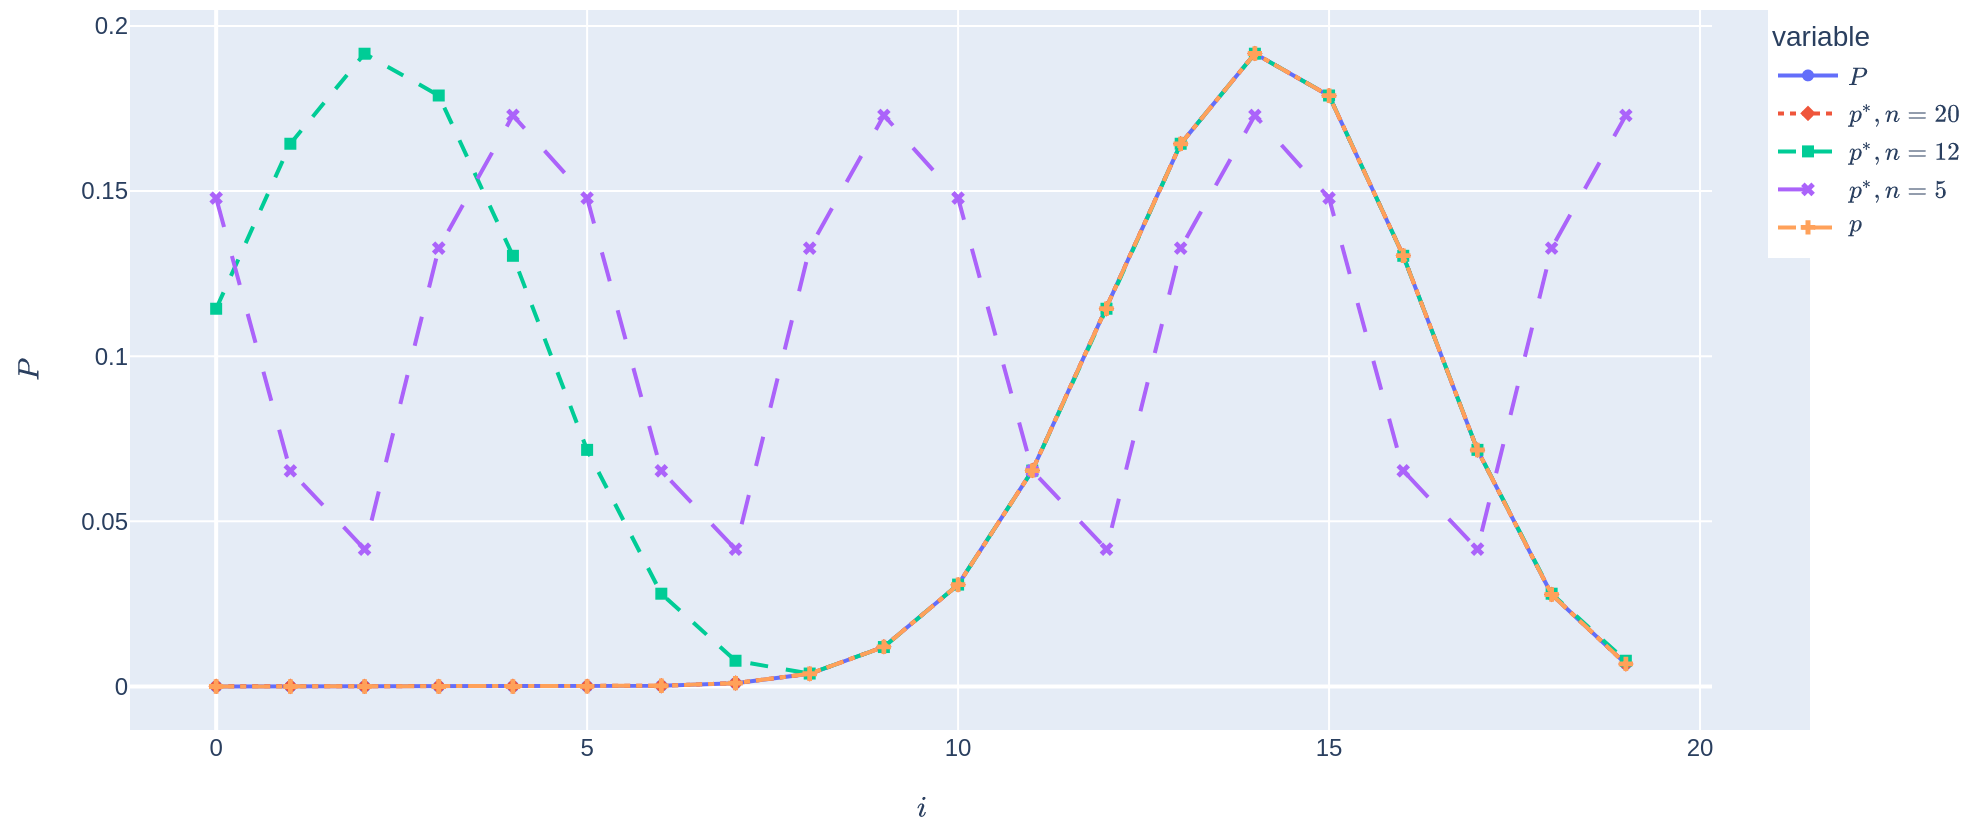
\includegraphics[height=6.8cm,width=\textwidth]{dft_figure1.png}
	\caption{Обращение характеристической функции} \label{dft_figure1}
\end{figure}

Вычисление было произведено на языке Python с заданными параметрами
\begin{equation*}
	n=20,p = 0.7,N = \{20,12\}.
\end{equation*}
Из рисунка \ref{dft_figure1} видно, что теоретическое биномиальное распределение $P$, результат обратного интегрального $p$ \eqref{int_dis_pos} и дискретного $p^*$ \eqref{dtf} преобразований совпадают при $N=20$. Однако, как показывает график, при неверном выборе шага дискретизации (в данном случае $N < n, N = 12$) распределение начинает искажаться, так как условие теоремы Котельникова \cite{ястребов2012дискретизация} не выполняется.
\subsection{Иллюстрация работы подхода на задаче теории массового обслуживания}\label{rq_3}
В данном разделе продемонстрируем эффективность предлагаемого подхода при реализации численных расчетов в задаче из \cite{blaginin2021approximation}. В данной работе получено асимптотическое приближение характеристической функции $h(u,t)$ числа обслуженных заявок в системе с повторными обращениями и вызываемыми заявками
\begin{equation}
	h(u,t)=\boldsymbol{R}e^{\boldsymbol{G}(u)t}\boldsymbol{E},
\end{equation}
которая при фиксированном $t$ является функцией только от $u$.

Здесь матрица $\boldsymbol{G}(u)$ содержит коэффициенты системы дифференциальных уравнений Колмогорова. Ее элементы выражаются через параметры модели. $\boldsymbol{R}$ --- вектор-строка, $\boldsymbol{E}$ --- единичный вектор-столбец.

Для вычисления характеристической функции необходимо вычислять матричную экспоненту $e^{\boldsymbol{G}(u)}$ , что безусловно делает задачу трудоемкой. Здесь матричную экспоненту вычисляем при помощи преобразования подобия матриц \cite{bronson1991matrix}:
\begin{equation*}
	e^{\boldsymbol{G}(u)}=\boldsymbol{T}(u)\cdot %\begin{bmatrix}
	%e^{ \Lambda_{1}(u)} & 0 &  0\\
	%0 & e^{ \Lambda_{2}(u)} & 0\\
	%0 & 0 &	e^{ \Lambda_{3}(u)}
	%\end{bmatrix}
	\boldsymbol{GJ}(u)
	\cdot \boldsymbol{T}(u)^{-1},
\end{equation*}
где $\boldsymbol{T}(u)$ --- матрица собственных векторов $\boldsymbol{G}(u)$, $\boldsymbol{GJ}(u)$ --- диагональная матрица собственных чисел $\Lambda_{n}$ матрицы $\boldsymbol{G}(u)$.

Вычисление распределения вероятностей числа обслуженных заявок в системе за некоторое фиксированное время t через интегрирование с помощью формулы \eqref{int_dis_pos} является, как уже было упомянуто, достаточно трудоемкой вычислительной задачей. Для решения этой проблемы предлагается воспользоваться формулой \eqref{dtf} ДПФ.

На рисунке \ref{dft_figure2z} видно, что результат дискретного преобразования Фурье ($p^*$) полностью совпадает с результатом вычисления при помощи интегрирования ($p$)
\begin{figure}[H]
	\centering
	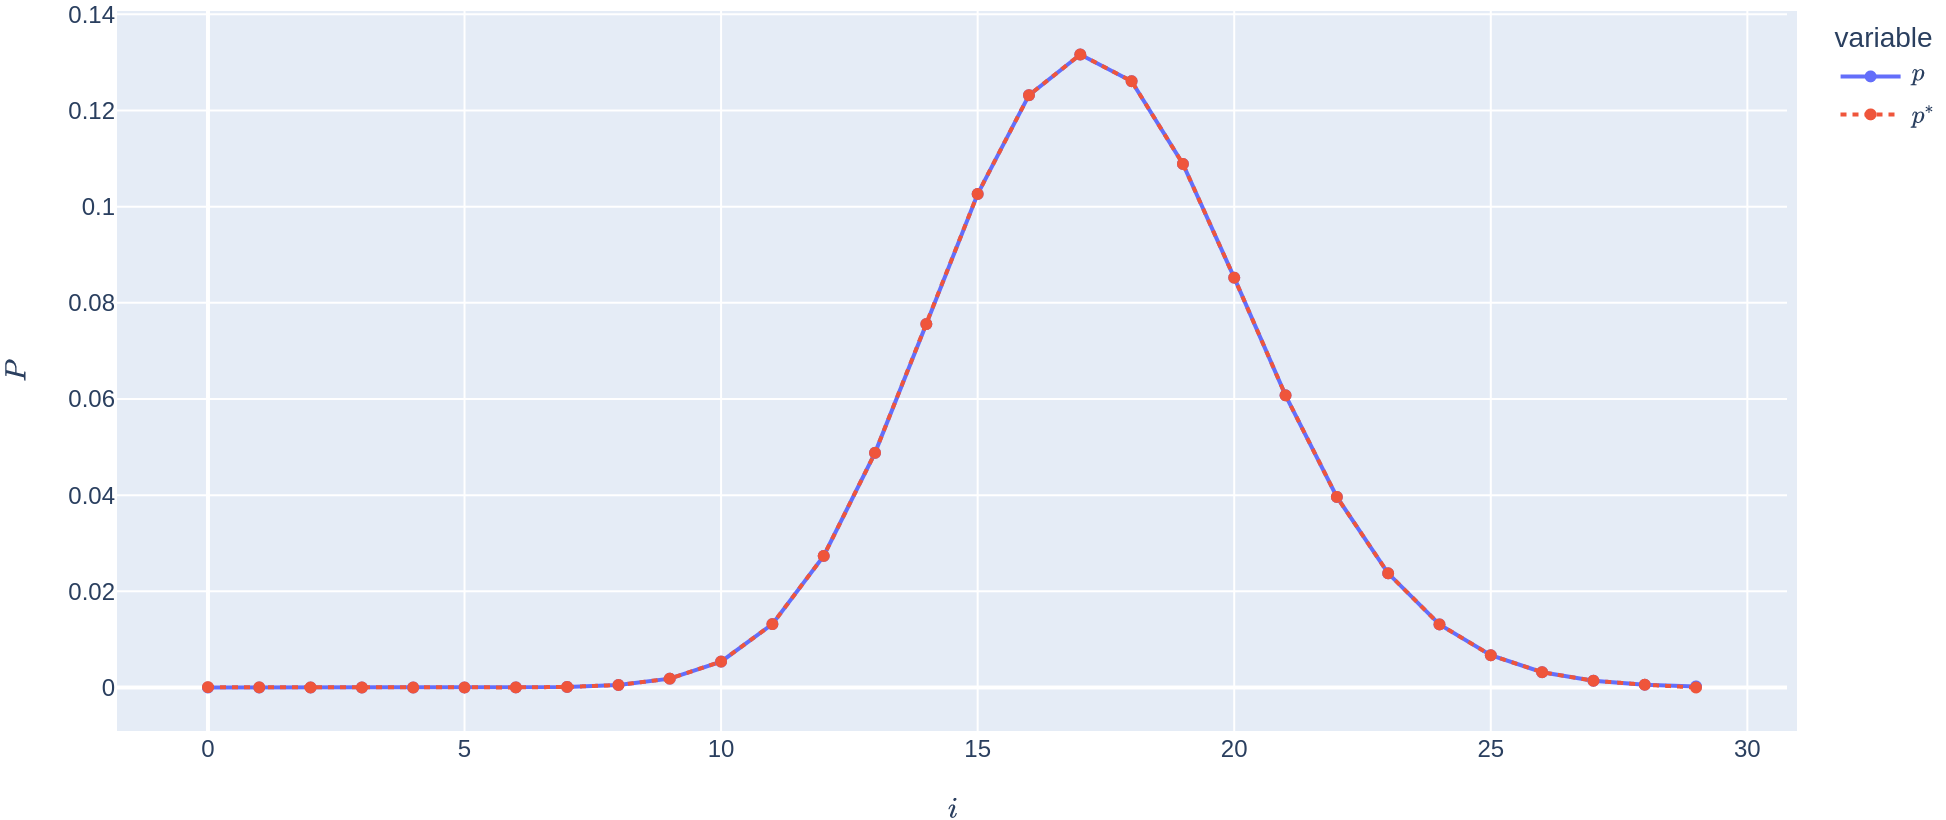
\includegraphics[scale=1,height=7cm,width=\textwidth]{dft_figure2.png}
	\caption{Сравнение распределений вероятностей, полученных с помощью интегрирования и ДПФ}
	\label{dft_figure2z}
\end{figure}

Для проверки скорости работы данного подхода к вычислению был проведен ряд тестов (400 запусков) со сравнением скорости работы алгоритмов и точности получаемого распределения при помощи расстояния Колмогорова \eqref{kdistance}.

В среднем ДПФ быстрее интегрирования более, чем в 100 раз, а среднее расстояние Колмогорова --- $4.16 \cdot 10^-6$.

Итак, предложенный метод позволяет в общем случае обращать характеристические функции гораздо более эффективно в сравнении с преобразованием Фурье, что в контексте разработанного программного комплекса позволяет быстрее вычислять асимптотические результаты и анализировать их, например, путем точечного сравнения распределений вероятности при помощи расстояния Колмогорова.

%\subsection{Вычисление коэффициента вариации MMPP}
%В данной работе одним из объектов изучения является вариация длин интервалов между моментами поступления заявок MMPP.

%Согласно \cite{вишневский2018стохастические}, вариация длин интервалов между моментами поступления заявок MMPP вычисляется как
%\begin{equation}
%	Var = \frac{\sqrt{v}}{Lg^{-1}},
%\end{equation}
%где $v$ --- дисперсия длин интервалов между моментами поступления групп запросов и рассчитывается как
%\begin{equation}
%	v = \frac{2Lg\cdot r \cdot (-D0)^{-1} \cdot E -1}{Lg^2},
%\end{equation}
%где вектор--строка $r$ --- стационарное распределение вероятностей процесса\\$\{k(t),n(t)\}$, $E$ --- единичный вектор--столбец размерности N, $Lg$ -- интенсивность %входящего потока
%\begin{equation} \label{eq_lg}
%	Lg = r\cdot \Lambda \cdot E,
%\end{equation}
%\begin{equation*}
%	D0 = Q - \Lambda - Q\cdot D,
%\end{equation*}
%где $D$ --- матрица, содержащая вероятности наступления события в потоке при смене его состояния.
\clearpage
 
\titleformat{\section}[block]
{\bfseries\centering}
{\thesection}
{1em}{}
\section*{\centering\normalsize ЗАКЛЮЧЕНИЕ}
\addcontentsline{toc}{section}{Заключение}
В рамках данной работы был рассмотрен ряд Марковских систем массового обслуживания с повторными вызовами и вызываемыми заявками, имеющих в качестве источника заявок простейший и MMPP--потоки. Согласно указанной цели исследования был выполнен ряд задач.

Были построены математические модели функционирования рассматриваемых узлов обработки запросов. В зависимости от типа системы, описывающий ее Марковский процесс имеет разную размерность. Так, для системы с одномерным выходящим потоком и простейшим входящим он будет трехмерным --- $\{k(t),i(t),m(t)\}$, при построении модели с разными типами заявок был добавлен процесс $m_{2}(t)$, а для системы с входящим потоком MMPP--потоком был добавлен процесс $n(t)$, описывающий состояние управляющей цепи MMPP. На основе Марковских процессов были составлены системы уравнений Колмогорова. Для нахождения характеристик выходящего потока был осуществлен переход к характеристическим функциям и применен метод асимптотического анализа в предельном условии большой задержки заявок на орбите. В результате были получены формулы (\ref{approximation_summary},\ref{approximation_twodim},\ref{approximation_twodim_map}) для вычисления асимптотического приближения характеристической функции числа заявок, окончивших обслуживание в системе к моменту времени $t$.

Для вычисления значений распределения вероятностей числа обслуженных заявок были получены формулы (\ref{distr_simple_summary},\ref{distr_simple_twodim},\ref{distr_map_twodim}), в которых используется преобразование подобия матриц для вычисления матричной экспоненты и обратное преобразование Фурье, позволяющее перейти от характеристической функции к явному виду распределения вероятностей. Помимо этого, в разделе \ref{corr_section} были приведены выкладки для вычисления коэффициента корреляции компонентов двумерного распределения при помощи полученных асимптотических приближений характеристической функции числа обслуженных заявок. Применение указанных формул позволило проводить анализ решений в системе компьютерной алгебры Mathcad и при заданных параметрах системы получать численные характеристики работы системы.

Для оценки применимости полученных асимптотических результатов был разработан и реализован программный продукт, позволяющий проводить имитационное моделирование рассматриваемых систем. В первую очередь, были выделены сущности, принадлежащие к предметной области работы. Далее, была построена объектная модель программы, позволяющая расширять набор используемых элементов теории массового обслуживания при помощи общего для них интерфейса, формализующего изменение состояния элемента при наступлении очередного события в модели. Процесс моделирования, заключающийся в регистрации моментов наступления событий, позволил проводить моделирование итеративно и регистрировать необходимые для анализа характеристики работы системы. Реализация программы представляет собой две составных части - библиотеку, реализованная с учетом построенной объектной модели и оболочку для ее использования с графическим пользовательским интерфейсом. Раздельная реализация дает возможность легко добавлять новый функционал к имеющемуся.  

Процесс работы с программой предусматривает два подхода. В первом случае, по умолчанию, моделирование производится в реальном времени с настраиваемым интервалом таймера, который отсчитывает проведение следующей итерации моделирования. Данный подход дает возможность пользователю получать результаты моделирования и проводить их предварительный анализ с помощью встроенных графических средств, таких как трехмерное представление распределения вероятностей с возможностью масштабирования и выделения необходимой области с отсечением. Второй способ позволяет быстро получить результаты моделирования для последующего анализа с помощью других программных средств, для чего реализована функция экспорта данных распределения вероятностей в текстовый формат. 

Имитационная модель была протестирована на стабильность получаемых результатов при помощи расстояния Колмогорова. В ходе эксперимента его значение не превышало 0.002, что говорит о высокой стабильности моделирования.

Из-за асимптотической природы полученных результатов встает вопрос об их применимости на практике в реальных системах, соответствующих рассматриваемых моделям. Для ее оценки была применена указанная имитационная модель и расстояние Колмогорова, показывающие, насколько соответствует эмпирическое распределение вероятностей предложенной модели. Расчеты показали, что при увеличении задержки заявок на орбите аналитические формулы дают более точное распределение вероятностей числа обслуженных заявок. Такой результат является закономерным ввиду того, что аналитические решения были получены при соответствующем асимптотическом условии, однако, даже при меньшей задержке заявок на орбите расчеты оказываются достаточно точными, чтобы их можно было применять на практике. Внимания требует так же распределение вероятностей, получаемое при большей загруженности системы. В таких условиях расчеты становятся еще более точными. В ходе проведенных численных экспериментов значение расстояния Колмогорова не превышало 0.066 --- данный результат был получен при увеличенной загрузке системы с MMPP--потоком при интенсивности возврата заявок с орбиты равной 10.

Для рассматриваемых систем был проведен численный анализ корреляции выходящих процессов, в ходе которого были выявлены некоторые закономерности изменения их корреляции при различных параметрах системы. В частности, при варьировании параметров для разных типов заявок коэффициент корреляции всегда меньше нуля и тем меньше, чем больше интенсивность поступления заявок, входящих либо вызываемых, в систему; в то время как при изменении параметров системы для одного типа заявок коэффициент корреляции принимает как положительные, так и отрицательные значения. Также были найдены параметры системы, при которых компоненты выходящего потока становятся независимыми. Эти результаты крайне важны для понимая функционирования выходящих процессов системы, однако для интерпретации этого открытия требуется дальнейшее исследование.

В конечном итоге, проведенное исследование позволяет применять полученные в ходе него аналитические решения и результаты численного анализа  для изучения функционирования и отладки реальных систем массового обслуживания \cite{deering1991icmp,nutt1982performance} с высокой точностью. Крайне важным и трудно исследуемым аспектом функционирования таких систем является выходящих поток обслуженных требований, поскольку он представляет собой характеристику работы системы в совокупности, а она, в свою очередь, зависит от других процессов, происходящих в рамках системы. Помимо этого, исследование выходящего потока требований и его характеристик является необходимым при построении телекоммуникационных сетей, поскольку обслуженные требования одного узла является входящими для другого, что для сетей значительного размера представляет собой еще более важный аспект проектирования.

Результаты проведенного исследования были представлены в качестве докладов и обсуждались на пяти международных конференциях:
\begin{itemize}
\item XIX Международная конференции по информационным технологиям и математическому моделированию имени А.Ф. Терпугова (ITMM) (май 2020, Томск);
\item VIII Международная молодежная научная конференция «Математическое и программное обеспечение информационных, технических и экономических систем» (май 2021, Томск);
\item VII Международная конференция «Математика, её приложения и математическое образование» (МПМО) (сентябрь 2020, Улан-Удэ);
\item V Международная конференции по стохастическим методам (ноябрь 2020, Москва);
\item VII Международная молодеждная научная конференция \textquote{Математическое и программное обеспечение информационных, технических и экономических систем} (май 2020, Томск).
\end{itemize}
Материалы, представленные в работе были опубликованы в трех сборниках материалов конференций \cite{itmm_2021,icsm,mpmo} и одной статье, индексируемой в Scopus \cite{blaginin2020two}. Также, для основного алгоритма имитационной модели было получено свидетельство о регистрации программы для ЭВМ \cite{evm}.
 \clearpage %Заключение
\bibliographystyle{ugost2008mod}
\addcontentsline{toc}{section}{Список использованной литературы}
\bibliography{refs.bib}\nocite{*}
\clearpage
%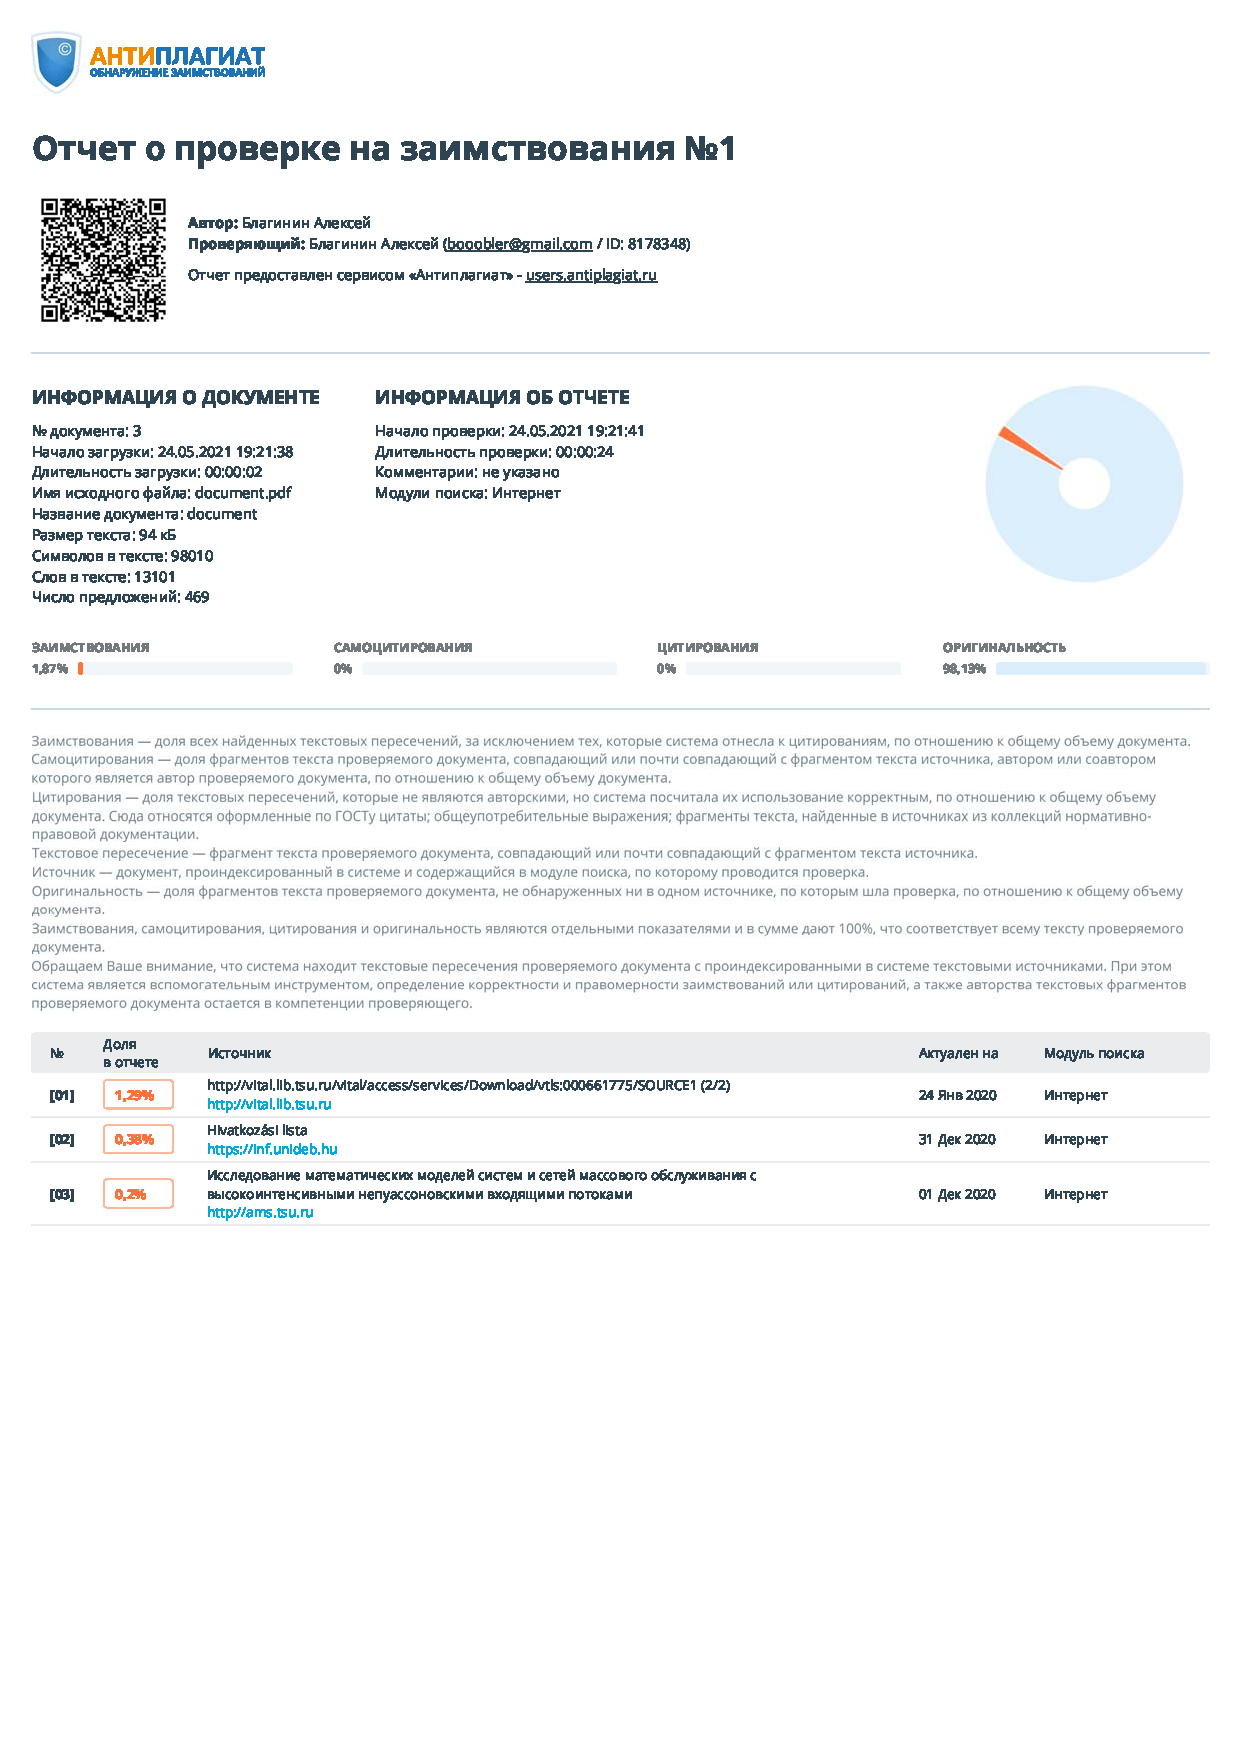
\includepdf[pagetemplate=1,scale=0.83,offset=0.75cm 0]{antiplagiat}
\end{document}